\RequirePackage{xcolor}
\documentclass[final,total,bgColor,slideColor,pdf,ps2pdf,default,noaccumulate]{prosper}

\usepackage{array}
\usepackage{xcolor}
\usepackage{longtable}
%\newcommand{\color}[2][]{}

\newcommand{\ii}{\includegraphics[scale=0.15]{/usr/share/texmf/tex/latex/prosper/red-bullet-on-white.ps}}
\newcommand{\qry}[1]{{\bf #1}}
\usepackage{../geostreams}

% This is used for multi-column tables
\newcommand{\PreserveBackslash}[1]{\let\temp=\\#1\let\\=\temp}
\let\PBS=\PreserveBackslash

%\usepackage{acronym}
%\newcommand{\acrodef}[3][]{}
\newcommand{\ac}[1]{#1}
\newcommand{\id}[1]{\ensuremath{#1}}
\newcommand{\dct}{\id{DCT}}
\newcommand{\key}{\id{key}}
\newcommand{\Xn}{\id{X_{-}}}
\newcommand{\Xx}{\id{X_{+}}}
\newcommand{\Yn}{\id{Y_{-}}}
\newcommand{\Yx}{\id{Y_{+}}}
\renewcommand{\Tn}{\id{T_{-}}}
\newcommand{\Tx}{\id{T_{+}}}
\newcommand{\A}{\id{A}}
\newcommand{\wxn}{\id{w_{x-}}}
\newcommand{\wxx}{\id{w_{x+}}}
\newcommand{\wyn}{\id{w_{y-}}}
\newcommand{\wyx}{\id{w_{y+}}}
\newcommand{\wt}{\id{w_{t}}}

\renewcommand{\r}{\id{r}}
\newcommand{\rid}{\id{r_{id}}}
\newcommand{\rin}{\id{r_{i-}}}
\newcommand{\rix}{\id{r_{i+}}}
\newcommand{\ryn}{\id{r_{1-}}}
\newcommand{\ryx}{\id{r_{1+}}}
\newcommand{\rxn}{\id{r_{2-}}}
\newcommand{\rxx}{\id{r_{2+}}}
\newcommand{\np}{\id{np}}
\newcommand{\npi}{\id{np_i}}
\newcommand{\npx}{\id{np_2}}
\newcommand{\npy}{\id{np_1}}



\newcommand{\Y}{$Y$}
\newcommand{\X}{$X$}
\newcommand{\cnx}{\id{cn_{x}}}
\newcommand{\cny}{\id{cn_{y}}}
%  \newcommand{\wxn}{\id{w_{x-}}}
%  \newcommand{\wxx}{\id{w_{x+}}}
%  \newcommand{\wyn}{\id{w_{y-}}}
%  \newcommand{\wyx}{\id{w_{y+}}}
%  \newcommand{\wt}{\id{w_{t}}}
%  \renewcommand{\r}{\id{r}}
%  \newcommand{\rid}{\id{r_{id}}}
%  \newcommand{\rin}{\id{r_{i-}}}
%  \newcommand{\rix}{\id{r_{i+}}}
%  \newcommand{\ryn}{\id{r_{1-}}}
%  \newcommand{\ryx}{\id{r_{1+}}}
%  \newcommand{\rxn}{\id{r_{2-}}}
%  \newcommand{\rxx}{\id{r_{2+}}}
%  \newcommand{\np}{\id{np}}
%  \newcommand{\npi}{\id{np_i}}
%  \newcommand{\npx}{\id{np_2}}
%  \newcommand{\npy}{\id{np_1}}

%\setlength{\unitlength}{1cm}

\title{Online Geospatial Image Databases}
\subtitle{The GeoStreams Project}
\author{Quinn Hart}
\institution{ CalSpace \\ University of California, Davis}
\email{qjhart@ucdavis.edu}

%
\date{July 2005}
%
\Logo{\includegraphics[width=1cm]{presentation/geostreams.eps}}
\DefaultTransition{Replace}
\slideCaption{Research Proposal \hfill qjhart@ucdavis.edu  }

\begin{document}

\maketitle

\begin{slide}[R]{GeoStreams} 
  \centering
  \vspace*{1.5cm}  
  \large{A framework to process multiple}
  \large{continuous queries against}
  \large{streaming, remotely-sensed,}
  \large{geospatial image data}

\end{slide}

\begin{slide}{Roadmap}
  \begin{Itemize}
  {\blue \item Overview and background}
  \item Models
  \item Query processing
  \item Operators
  \item The dynamic cascade tree
  \item Conclusions and work plan
  \end{Itemize}
\end{slide}

% Identify were my interests lie.
% Focus on the Query optimization issues
\begin{slide}{Areas of Research}
  \begin{Itemize}
  \item Geo-spatial image databases
    \begin{Itemize}
    \item Satellite imagery / raster databases
    \item \emph{Earth Observing System} requirements
    \item Meteorological data growing exponentially
    {\blue \item Little research on streaming data }
    \end{Itemize}
  \item Data Stream Management Systems (DSMSs)
    \begin{Itemize}
    \item Current studies involve simple tuples
    \item Much interest in spatio-temporal data
    \item Extensions to SQL
    {\blue \item Little research on complex data like images}
    \end{Itemize}
  \item Meteorological satellite image processing
  \end{Itemize}
\end{slide}

\begin{slide}{Overview}
%  figs/version is too small, and not in color
%  \begin{picture}(0,0)%
\includegraphics{figs/overview.fig.eps}%
\end{picture}%
\setlength{\unitlength}{4144sp}%
%
\begingroup\makeatletter\ifx\SetFigFontNFSS\undefined%
\gdef\SetFigFontNFSS#1#2#3#4#5{%
  \reset@font\fontsize{#1}{#2pt}%
  \fontfamily{#3}\fontseries{#4}\fontshape{#5}%
  \selectfont}%
\fi\endgroup%
\begin{picture}(3431,2004)(79,-1198)
\put(136,322){\makebox(0,0)[lb]{\smash{{\SetFigFontNFSS{5}{6.0}{\familydefault}{\mddefault}{\updefault}{\color[rgb]{0,0,0}connect}%
}}}}
\put(2858,-421){\makebox(0,0)[lb]{\smash{{\SetFigFontNFSS{6}{7.2}{\familydefault}{\mddefault}{\updefault}{\color[rgb]{0,0,0}Stream}%
}}}}
\put(2858,-556){\makebox(0,0)[lb]{\smash{{\SetFigFontNFSS{6}{7.2}{\familydefault}{\mddefault}{\updefault}{\color[rgb]{0,0,0}Generator}%
}}}}
\put(136,-308){\makebox(0,0)[lb]{\smash{{\SetFigFontNFSS{5}{6.0}{\familydefault}{\mddefault}{\updefault}{\color[rgb]{0,0,0}connect}%
}}}}
\put(136,-893){\makebox(0,0)[lb]{\smash{{\SetFigFontNFSS{5}{6.0}{\familydefault}{\mddefault}{\updefault}{\color[rgb]{0,0,0}connect}%
}}}}
\put(1621,-196){\rotatebox{270.0}{\makebox(0,0)[lb]{\smash{{\SetFigFontNFSS{6}{7.2}{\familydefault}{\mddefault}{\updefault}{\color[rgb]{0,0,0}Parser}%
}}}}}
\put(2206,-196){\makebox(0,0)[lb]{\smash{{\SetFigFontNFSS{6}{7.2}{\familydefault}{\mddefault}{\updefault}{\color[rgb]{0,0,0}Optimization}%
}}}}
\put(1621,-691){\rotatebox{270.0}{\makebox(0,0)[lb]{\smash{{\SetFigFontNFSS{6}{7.2}{\familydefault}{\mddefault}{\updefault}{\color[rgb]{0,0,0}Delivery}%
}}}}}
\put(1486, 29){\makebox(0,0)[lb]{\smash{{\SetFigFontNFSS{6}{7.2}{\familydefault}{\mddefault}{\updefault}{\color[rgb]{0,0,0}\acs{DSMS} Server}%
}}}}
\put(2138,-1066){\makebox(0,0)[lb]{\smash{{\SetFigFontNFSS{6}{7.2}{\familydefault}{\mddefault}{\updefault}{\color[rgb]{0,0,0}Execution}%
}}}}
\put(1396,704){\makebox(0,0)[lb]{\smash{{\SetFigFontNFSS{6}{7.2}{\familydefault}{\mddefault}{\updefault}{\color[rgb]{0,0,0}Weather Satellites}%
}}}}
\end{picture}%

  \begin{picture}(0,0)%
\includegraphics{figs/overview.fig.eps}%
\end{picture}%
\setlength{\unitlength}{4144sp}%
%
\begingroup\makeatletter\ifx\SetFigFontNFSS\undefined%
\gdef\SetFigFontNFSS#1#2#3#4#5{%
  \reset@font\fontsize{#1}{#2pt}%
  \fontfamily{#3}\fontseries{#4}\fontshape{#5}%
  \selectfont}%
\fi\endgroup%
\begin{picture}(3431,2004)(79,-1198)
\put(136,322){\makebox(0,0)[lb]{\smash{{\SetFigFontNFSS{5}{6.0}{\familydefault}{\mddefault}{\updefault}{\color[rgb]{0,0,0}connect}%
}}}}
\put(2858,-421){\makebox(0,0)[lb]{\smash{{\SetFigFontNFSS{6}{7.2}{\familydefault}{\mddefault}{\updefault}{\color[rgb]{0,0,0}Stream}%
}}}}
\put(2858,-556){\makebox(0,0)[lb]{\smash{{\SetFigFontNFSS{6}{7.2}{\familydefault}{\mddefault}{\updefault}{\color[rgb]{0,0,0}Generator}%
}}}}
\put(136,-308){\makebox(0,0)[lb]{\smash{{\SetFigFontNFSS{5}{6.0}{\familydefault}{\mddefault}{\updefault}{\color[rgb]{0,0,0}connect}%
}}}}
\put(136,-893){\makebox(0,0)[lb]{\smash{{\SetFigFontNFSS{5}{6.0}{\familydefault}{\mddefault}{\updefault}{\color[rgb]{0,0,0}connect}%
}}}}
\put(1621,-196){\rotatebox{270.0}{\makebox(0,0)[lb]{\smash{{\SetFigFontNFSS{6}{7.2}{\familydefault}{\mddefault}{\updefault}{\color[rgb]{0,0,0}Parser}%
}}}}}
\put(2206,-196){\makebox(0,0)[lb]{\smash{{\SetFigFontNFSS{6}{7.2}{\familydefault}{\mddefault}{\updefault}{\color[rgb]{0,0,0}Optimization}%
}}}}
\put(1621,-691){\rotatebox{270.0}{\makebox(0,0)[lb]{\smash{{\SetFigFontNFSS{6}{7.2}{\familydefault}{\mddefault}{\updefault}{\color[rgb]{0,0,0}Delivery}%
}}}}}
\put(1486, 29){\makebox(0,0)[lb]{\smash{{\SetFigFontNFSS{6}{7.2}{\familydefault}{\mddefault}{\updefault}{\color[rgb]{0,0,0}\acs{DSMS} Server}%
}}}}
\put(2138,-1066){\makebox(0,0)[lb]{\smash{{\SetFigFontNFSS{6}{7.2}{\familydefault}{\mddefault}{\updefault}{\color[rgb]{0,0,0}Execution}%
}}}}
\put(1396,704){\makebox(0,0)[lb]{\smash{{\SetFigFontNFSS{6}{7.2}{\familydefault}{\mddefault}{\updefault}{\color[rgb]{0,0,0}Weather Satellites}%
}}}}
\end{picture}%

\end{slide}

\begin{slide}[R]{\emph{GeoStreams} Objectives}
  \begin{Itemize}

% Identify Data Model, Query
  \item Image specific data model and query framework

  \item Imagery operations
 
  \item Query optimizations

    \begin{Itemize}
    \item Logical rewrites
    \item Multiple queries
    \end{Itemize}

  \item Operator implementations

    \begin{Itemize}
    \item Special characteristics of streaming images
    \end{Itemize}

  \item Convenient interfaces

  \end{Itemize}
\end{slide}

\begin{slide}{GOES Weather Satellite}
  % figs version not complete
  %\begin{picture}(0,0)%

\includegraphics{figs/motivation-goes.fig.eps}%
\end{picture}%
\setlength{\unitlength}{4144sp}%
%
\begingroup\makeatletter\ifx\SetFigFont\undefined%
\gdef\SetFigFont#1#2#3#4#5{%
  \reset@font\fontsize{#1}{#2pt}%
  \fontfamily{#3}\fontseries{#4}\fontshape{#5}%
  \selectfont}%
\fi\endgroup%
\begin{picture}(1342,1342)(9,-503)
\end{picture}%

  \begin{picture}(0,0)%

\includegraphics{figs/motivation-goes.fig.eps}%
\end{picture}%
\setlength{\unitlength}{4144sp}%
%
\begingroup\makeatletter\ifx\SetFigFont\undefined%
\gdef\SetFigFont#1#2#3#4#5{%
  \reset@font\fontsize{#1}{#2pt}%
  \fontfamily{#3}\fontseries{#4}\fontshape{#5}%
  \selectfont}%
\fi\endgroup%
\begin{picture}(1342,1342)(9,-503)
\end{picture}%

\end{slide}

\begin{slide}[R]{Image Algebra for Raster Images}

  Image algebra is a multi-valued formalism for image manipulation

  \begin{Itemize}
  \item Point sets [\ps{X}]
    \begin{Itemize}
    \item Spatio-temporal points in the image.
    \item Time goes on and on ...
    \end{Itemize}
  \item Value sets [\vs{F}]
    \begin{Itemize}
    \item Encompass values associated with the points in a point set
%
%    \item Homogeneous sets like integers or real numbers.
    \end{Itemize}
  \item Images [\im{a}]
    \begin{Itemize}
    \item Function from $\ps{X} \to \vs{F}$,  $\im{a} \in \imType{F}{X}$
    \item Relation $\im{a} = \{(\pt{x},\im{a}(\pt{x})) : \pt{x}
      \in \ps{X}\}$ \\ \text {where $(\pt{x},\im{a}(\pt{x}))$ is a
        \emph{pixel}}
    \end{Itemize}
  \end{Itemize}
\end{slide}

\begin{slide}{Image Operations}

\centering 
\psset{unit=0.2}
  \begin{minipage}[t]{3.75cm}
    \centering
    \begin{pspicture}(10,10)
      \extent(0,0)(4,4)
      \extent(6,0)(10,4)
      \extent(3,5)(7,9)
      \roi(4,6)(5,7){}
      \pscurve[doubleline=true]{->}(1.5,1.5)(3,2)(4.5,6.5)
      \pscurve[doubleline=true]{->}(7.5,1.5)(5,2)(4.5,6.5)
    \end{pspicture}
    
\emph{Induced operations}

$\im{a} + \im{b}$

  \end{minipage}
\quad
  \begin{minipage}[t]{3.75cm}
    \centering
    \begin{FramePic}[10,10]
      \roi(2,2)(7,7){$\ps{X}$}
    \end{FramePic}

    \emph{Image restrictions} 

    $\im{a}|_\ps{X}$

  \end{minipage}

%\vspace*{1cm}

  \begin{minipage}[t]{3.75cm}
    \centering
    \begin{pspicture}(2,2)
%      {\psset{unit=0.2}\extent(0,0)(6,6)}
      {\extent(0,0)(6,6)}
      { \psset{unit=5.0}
        \SpecialCoor
        \newpsstyle{pc}{fillstyle=solid,fillcolor=white,linecolor=lightgray,origin={2,-1.8}}
        \pspolygon[style=pc](2;0)(4;0)(4;-24)(2;-24)(2;0)
        \psline[style=pc](2;-6)(4;-6)
        \psline[style=pc](2;-12)(4;-12)
        \psline[style=pc](2;-18)(4;-18)
        \psline[style=pc](2.5;0)(2.5;-24)
        \psline[style=pc](3;0)(3;-24)
        \psline[style=pc](3.5;0)(3.5;-24)
        \pscurve[doubleline=true]{->}(0.1,0.1)(.2,.7)(.5,.9)
        }
    \end{pspicture}

\emph{Spatial transformations}

$\im{a} \circ f$

  \end{minipage}
\quad
  \begin{minipage}[t]{3.75cm}
    \centering
    \begin{pspicture}(10,10)
      \extent(0,0)(6,6)
      \roi(0,0)(3,3){}
      \extent(4,4)(10,10)
      \roi(4,4)(10,10){}
      \roi(5,5)(6,6){}
      \pscurve[doubleline=true]{->}(1.5,1.5)(3,2)(5.5,5,5)
    \end{pspicture}
    
\emph{Neighborhood operations}

$\im{a} \bigoplus N$

  \end{minipage}

\end{slide}


\begin{slide}{Queries}

  Queries $\equiv$ expressions, $(\im{IR}/\im{VIS}) \circ UTM |_{\ps{CA}}$
  \begin{Itemize}
  \item $\im{IR}/\im{VIS}$ is an index
  \item $\circ UTM$ converts coordinate system
  \item $|_{\ps{CA}}$ selects California
  \item Questions specifying $UTM, \ps{CA}$ ?
  \end{Itemize}
      
  OpenGIS Web Map Service queries
  \begin{Itemize}
  \item Well known, simple, important queries
  \item $\im{c} \bigoplus N \circ f |_\ps{X}$ \\
    where \im{c}, $N$, $f$, and \ps{X} are specified in a simple
    standard way
  \item \im{c} could still be a function $(\im{a}-\im{b})/(\im{a}+\im{b})$
  \end{Itemize}
\end{slide}

\begin{slide}{Reference Queries}
  \vspace*{-0.3cm}
  \centering
  \begin{tabular}{l|c|>{\tiny \PBS\raggedright\hspace{0pt}}p{5cm}}
    
    Identifier & Expression & Description \\

    \hline
    \hline

    \qry{Vis} & $\im{VIS}$ & \ac{GOES} satellite visible channel; all data \\

    \hline

    \qry{VisNA} & $\im{VIS}|_{\ps{NA}}$ & Visible \ac{GOES} data for North America \\

    \hline

    \qry{VisCA} & $\im{VIS}|_{\ps{CA}}$ & Visible \ac{GOES} data for California \\

    \hline

    \qry{VisNA@t} & $\im{VIS}|_{\ps{CA}}|_\ps{@t}$ & Visible GOES data for NA, at time, \pt{t}, every day \\

    \hline

    \qry{NdviNA} & $\frac{\im{IR}-\im{VIS}}{\im{VIS}+\im{IR}}|_{\ps{NA}} $ & NDVI, $f(Vis,IR)$, for North America \\

    \hline

    \qry{VisCA-UTM} & $\im{VIS} \circ UTM |_{\ps{CA}}$ & Visible data for California, projected to UTM \\

    \hline

    \qry{VisCA-UTM$<\pt{d}$} & $\im{VIS} \circ UTM |_{\ps{CA}}|_{\ps{<\pt{d}}}$ &  Visible data for California, projected to UTM, until ending date, \pt{d} \\

    \hline

    \qry{Vis$>$v} & $Vis\||_{vis(x) > v}$ & Visible data, where the \emph{pixel values} $>v$ \\ 

    \hline

    \qry{CloudsCA} & & Complete cloud cover algorithm \\

  \end{tabular}
\end{slide}

\begin{slide}{GOES Cloud Cover}
  \centering
  \vspace{-0.5cm}
  \scalebox{1.0}{\begin{picture}(0,0)%
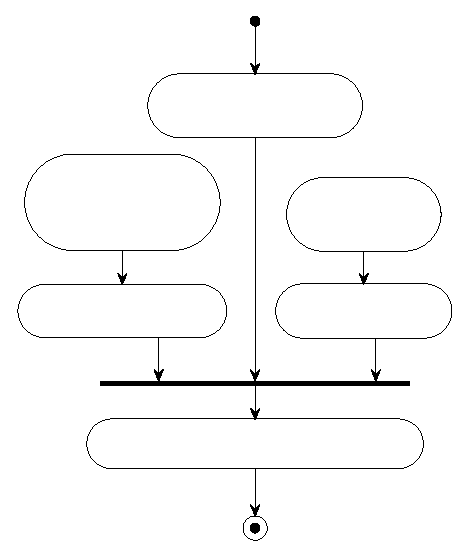
\includegraphics{figs/cloud_cover.atd.fig.eps}%
\end{picture}%
\setlength{\unitlength}{3947sp}%
%
\begingroup\makeatletter\ifx\SetFigFont\undefined%
\gdef\SetFigFont#1#2#3#4#5{%
  \reset@font\fontsize{#1}{#2pt}%
  \fontfamily{#3}\fontseries{#4}\fontshape{#5}%
  \selectfont}%
\fi\endgroup%
\begin{picture}(3491,4199)(24,-3369)
\put(870,-464){\makebox(0,0)[b]{\smash{{\SetFigFont{6}{7.2}{\rmdefault}{\mddefault}{\updefault}Get List of}}}}
\put(870,-643){\makebox(0,0)[b]{\smash{{\SetFigFont{6}{7.2}{\rmdefault}{\mddefault}{\updefault}All images at}}}}
\put(870,-793){\makebox(0,0)[b]{\smash{{\SetFigFont{6}{7.2}{\rmdefault}{\mddefault}{\updefault}same time for}}}}
\put(870,-957){\makebox(0,0)[b]{\smash{{\SetFigFont{6}{7.2}{\rmdefault}{\mddefault}{\updefault}last 2 weeks}}}}
\put(870,-1517){\makebox(0,0)[b]{\smash{{\SetFigFont{6}{7.2}{\rmdefault}{\mddefault}{\updefault}$alb_T$ =}}}}
\put(870,-1676){\makebox(0,0)[b]{\smash{{\SetFigFont{6}{7.2}{\rmdefault}{\mddefault}{\updefault}min(above images)}}}}
\put(2801,-638){\makebox(0,0)[b]{\smash{{\SetFigFont{6}{7.2}{\rmdefault}{\mddefault}{\updefault}Get 9x9}}}}
\put(2801,-817){\makebox(0,0)[b]{\smash{{\SetFigFont{6}{7.2}{\rmdefault}{\mddefault}{\updefault}average of}}}}
\put(2801,-981){\makebox(0,0)[b]{\smash{{\SetFigFont{6}{7.2}{\rmdefault}{\mddefault}{\updefault}image}}}}
\put(2801,-1498){\makebox(0,0)[b]{\smash{{\SetFigFont{6}{7.2}{\rmdefault}{\mddefault}{\updefault}Get Maximum}}}}
\put(2801,-1676){\makebox(0,0)[b]{\smash{{\SetFigFont{6}{7.2}{\rmdefault}{\mddefault}{\updefault}Value of Image}}}}
\put(1932,-2656){\makebox(0,0)[b]{\smash{{\SetFigFont{6}{7.2}{\rmdefault}{\mddefault}{\updefault}$N= (vis_T-alb_T)/(Max-alb_T)$}}}}
\put(1932,125){\makebox(0,0)[b]{\smash{{\SetFigFont{6}{7.2}{\rmdefault}{\mddefault}{\updefault}$vis_T$, is Image}}}}
\put(1932,-34){\makebox(0,0)[b]{\smash{{\SetFigFont{6}{7.2}{\rmdefault}{\mddefault}{\updefault}at Time,$T$}}}}
\end{picture}%
}
\end{slide}

\newcommand{\Tb}[1]{ \Tr{\psframebox{\rule{0pt}{9pt}#1}} }

\begin{slide}{Optimization Example}
  \centering
  \vspace*{1.5cm}
  \begin{tabular}{cc}
%     \pstree[treemode=U,nodesep=2pt,levelsep=30pt]{\TR{Q}}{
%       \pstree[treemode=U]{\Tb{$|_{NA}$}}{
%         \pstree[treemode=U]{\Tcircle{/}}{
%           \pstree[treemode=U]{\Tcircle{+}}{
%             \TR[name=VIS]{\im{VIS}}
%             \TR[name=IR]{\im{IR}}
%           }
%           \Tcircle[name=minus]{-}
%           \ncline{VIS}{minus}
%           \ncline{IR}{minus}
%         }
%       }
%     }
%     &
    \pstree[treemode=U,nodesep=2pt,levelsep=30pt]{\TR{Q}}{
      \pstree[treemode=U]{\Tb{$|_{NA}$}}{
        \pstree[treemode=U]{\Tb{$\im{IR}/\im{VIS}$}}{
          \TR[name=VIS]{\im{VIS}}
          \TR[name=IR]{\im{IR}}
        }
      }
    }
    &
    \pstree[treemode=U,nodesep=2pt,levelsep=30pt]{\TR{Q}}{
      \pstree[treemode=U]{\Tb{$\im{IR}/\im{VIS}$}}{
        \pstree[treemode=U]{\Tb{$|_{NA}$}}{
          \TR[name=VIS]{\im{VIS}}
        }
        \pstree[treemode=U]{\Tb{$|_{NA}$}}{
          \TR[name=IR]{\im{IR}}
        }
      }
    } \\
%&
%    \pstree[treemode=U,nodesep=2pt,levelsep=30pt]{\TR{Q}}{
%      \pstree[treemode=U]{\Tb{$|_{NA}$}}{
%        \pstree[treemode=U]{\Tb{$\im{IR} \circ UTM$}}{
%          \TR[name=IR]{\im{IR}}
%        }
%      }
%    }\\
%&
%    \pstree[treemode=U,nodesep=2pt,levelsep=30pt]{\TR{Q}}{
%        \pstree[treemode=U]{\Tb{$\im{IR} \circ UTM$}}{
%          \pstree[treemode=U]{\Tb{$|_{f(\im{NA})}$}}{
%          \TR[name=IR]{\im{IR}}
%        }
%      }
%    }\\
    $(\im{IR}/\im{VIS})|_{\ps{NA}} $ &
    $(\im{VIS}|_{\ps{NA}})/(\im{IR}|_{\ps{NA}})$
%    $\frac{\im{IR}-\im{VIS}}{\im{VIS}+\im{IR}}|_{\ps{NA}} $ &
%    $\frac{\im{IR}-\im{VIS}}{\im{VIS}+\im{IR}}|_{\ps{NA}} $ &
  \end{tabular}
\end{slide}

\begin{slide}{Multiple Queries}
\centering
\begin{picture}(0,0)%
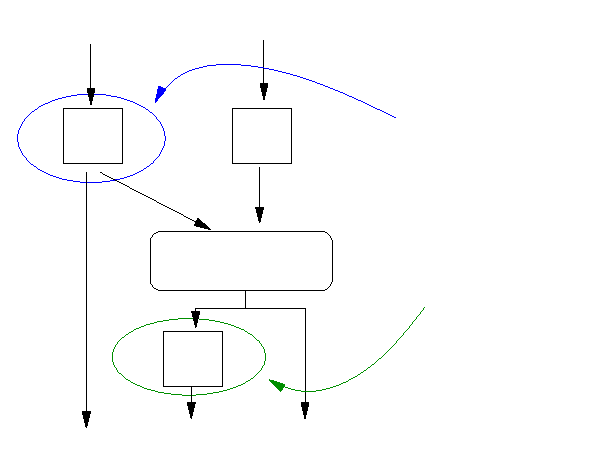
\includegraphics{figs/multi-op.fig.eps}%
\end{picture}%
\setlength{\unitlength}{4144sp}%
%
\begingroup\makeatletter\ifx\SetFigFont\undefined%
\gdef\SetFigFont#1#2#3#4#5{%
  \reset@font\fontsize{#1}{#2pt}%
  \fontfamily{#3}\fontseries{#4}\fontshape{#5}%
  \selectfont}%
\fi\endgroup%
\begin{picture}(4363,3344)(-322,-2506)
\put(1441,-106){\makebox(0,0)[lb]{\smash{{\SetFigFont{9}{10.8}{\familydefault}{\mddefault}{\updefault}{\color[rgb]{0,0,0}$|_\ps{X}$}%
}}}}
\put(991,-1051){\makebox(0,0)[lb]{\smash{{\SetFigFont{9}{10.8}{\familydefault}{\mddefault}{\updefault}{\color[rgb]{0,0,0}$\im{IR} / \im{VIS}$}%
}}}}
\put(901,-1816){\makebox(0,0)[lb]{\smash{{\SetFigFont{9}{10.8}{\familydefault}{\mddefault}{\updefault}{\color[rgb]{0,0,0}$|_\ps{X}$}%
}}}}
\put(136,-106){\makebox(0,0)[lb]{\smash{{\SetFigFont{9}{10.8}{\familydefault}{\mddefault}{\updefault}{\color[rgb]{0,0,0}$|_\ps{X}$}%
}}}}
\put(1043,-2145){\makebox(0,0)[lb]{\smash{{\SetFigFont{9}{10.8}{\familydefault}{\mddefault}{\updefault}{\color[rgb]{0,0,0}\ps{CA}}%
}}}}
\put(591,-480){\makebox(0,0)[lb]{\smash{{\SetFigFont{9}{10.8}{\familydefault}{\mddefault}{\updefault}{\color[rgb]{0,0,0}\ps{NA}}%
}}}}
\put(1530,-619){\makebox(0,0)[lb]{\smash{{\SetFigFont{9}{10.8}{\familydefault}{\mddefault}{\updefault}{\color[rgb]{0,0,0}\ps{NA}}%
}}}}
\put(245,-688){\makebox(0,0)[lb]{\smash{{\SetFigFont{9}{10.8}{\familydefault}{\mddefault}{\updefault}{\color[rgb]{0,0,0}\ps{CA}}%
}}}}
\put(1400,715){\makebox(0,0)[lb]{\smash{{\SetFigFont{9}{10.8}{\familydefault}{\mddefault}{\updefault}{\color[rgb]{0,0,0}\im{IR}}%
}}}}
\put( 42,715){\makebox(0,0)[lb]{\smash{{\SetFigFont{9}{10.8}{\familydefault}{\mddefault}{\updefault}{\color[rgb]{0,0,0}\im{VIS}}%
}}}}
\put( 91,-2446){\makebox(0,0)[lb]{\smash{{\SetFigFont{9}{10.8}{\familydefault}{\mddefault}{\updefault}{\color[rgb]{0,0,0}\im{Q}}%
}}}}
\put(901,-2446){\makebox(0,0)[lb]{\smash{{\SetFigFont{9}{10.8}{\familydefault}{\mddefault}{\updefault}{\color[rgb]{0,0,0}\im{R}}%
}}}}
\put(1756,-2446){\makebox(0,0)[lb]{\smash{{\SetFigFont{9}{10.8}{\familydefault}{\mddefault}{\updefault}{\color[rgb]{0,0,0}\im{S}}%
}}}}
\put(2611,-106){\makebox(0,0)[lb]{\smash{{\SetFigFont{12}{14.4}{\familydefault}{\mddefault}{\updefault}{\color[rgb]{0,0,1}Shared Operators}%
}}}}
\put(2656,-1351){\makebox(0,0)[lb]{\smash{{\SetFigFont{12}{14.4}{\familydefault}{\mddefault}{\updefault}{\color[rgb]{0,.56,0}Ordering}%
}}}}
\put(2656,-1096){\makebox(0,0)[lb]{\smash{{\SetFigFont{12}{14.4}{\familydefault}{\mddefault}{\updefault}{\color[rgb]{0,.56,0}Better Operator}%
}}}}
\put(2161,659){\makebox(0,0)[lb]{\smash{{\SetFigFont{12}{14.4}{\familydefault}{\mddefault}{\updefault}{\color[rgb]{0,0,0}Incoming Streams}%
}}}}
\put(2296,-2491){\makebox(0,0)[lb]{\smash{{\SetFigFont{12}{14.4}{\familydefault}{\mddefault}{\updefault}{\color[rgb]{0,0,0}Continuous Queries}%
}}}}
\end{picture}%
  
\end{slide}

\begin{slide}[R]{Example Application}
  \includegraphics[width=12cm]{presentation/screenshot.eps}
\end{slide}

% \begin{slide}{Roadmap}
%   \begin{Itemize}
%   { \tiny \item Overview and Background}
%   {\blue \item Models
%   \begin{Itemize}
%   \item Data Model
%     \begin{Itemize}
%     \item Point Set Order
%     \item Geographic Point Sets
%     \item Geostream Images   
%     \end{Itemize}
%   \item Query Model
%     \begin{Itemize}
%     \item Operator Modifications
%     \item Algebraic Rewriting Rules
%     \end{Itemize}
%   \end{Itemize} }
%   { \tiny \item Query Processing
%   \item Operators
%   \item The Dynamic Cascade Tree
%   \item Conclusions and Work Plan }
%   \end{Itemize}
% \end{slide}

\begin{slide}{Roadmap - Models}
  { \tiny \ii Overview and background }
    \begin{Itemize}
  \item Models \\ {\blue Objectives / Contributions }
    \begin{Itemize}
    \item Refine image algebra to make it consistent with streaming
      RSI data; point sets and operators
    \item Examine image algebra identities for expression rewriting
    \end{Itemize}
  {\blue Related work }
    \begin{Itemize}
    \item Image algebra, geographic information systems
    \end{Itemize}
%  {\blue TODO }
%    \begin{Itemize}
%    \item More investigation of requirements for image algebra
%      expression rewriting
%    \end{Itemize}
  \end{Itemize}
  { \tiny \ii Query processing \ii Operators \ii Dynamic cascade tree \ii Conclusions }
\end{slide}

\begin{slide}{Point Set Organization - Row Order}
  \centering
  {
    \psset{unit=0.3}
    
    \begin{tabular}{cc}
      {
        \begin{FramePic}[10,10]
        \pscurve[dotstyle=x,showpoints=true]{->}%
        (1.4,1.5)(1.6,2.6)(1.5,3.7)(1.5,4.8)(1.3,5.9)(1.5,7.0)(1.6,8.2)(1.7,9.3) %
        (3.2,9.5)(3.0,8.6)(3.0,7.4)(2.9,6.5)(2.8,4.5)(2.6,3.5)(2.8,2.5)(3.2,1.5)%
        (4.4,1.5)(4.6,2.6)(4.5,3.7)(4.5,4.8)(4.3,5.9)(4.5,7.0)(4.6,8.2)(4.7,9.3) %
        (6.2,9.5)(6.0,8.6)(6.0,7.4)(5.9,6.5)(5.6,5.5)(5.8,2.5)(6.2,1.5)%
        (8.2,1.3)(8.5,2.1)(8.5,3.4)(8.6,4.5)(8.4,5.3)(8.3,7.4)(8.4,8.8)
      \end{FramePic}} & 
 {
    \begin{FramePic}[10,10]
     \psline[linecolor=gray]{->}(0.5,9.5)(9.5,9.5)
   \psline[linecolor=gray]{->}(0.5,8.5)(9.5,8.5)
   \psline[linecolor=gray]{->}(0.5,7.5)(9.5,7.5)
   \psline[linecolor=gray]{->}(0.5,6.5)(9.5,6.5)
   \psline[linecolor=gray]{->}(0.5,5.5)(9.5,5.5)
   \psline[linecolor=gray]{->}(0.5,4.5)(9.5,4.5)
   \psline[linecolor=gray]{->}(0.5,3.5)(9.5,3.5)
   \psline[linecolor=gray]{->}(0.5,2.5)(9.5,2.5)
   \psline[linecolor=gray]{->}(0.5,1.5)(9.5,1.5)
   \psline[linecolor=gray]{->}(0.5,0.5)(9.5,0.5)
 \end{FramePic}} \\
{\tiny non-uniform } & {\tiny row-scan order lattice } \\
\end{tabular}
}
\vspace*{0.5cm}
\includegraphics[width=8cm]{presentation/pointsets.eps}

\end{slide}


% COMBINE THESE SLIDES

\begin{slide}{Geographic Point Set Attributes}
  \centering
  \begin{Itemize}
  \item Projection Definition \\
    { \fontsize{6}{6}\selectfont
\begin{verbatim}
  PROJCS["UTM 17 (WGS84) in northern hemisphere",
      GEOGCS["WGS 84",
          DATUM["WGS_1984",....]]]
\end{verbatim}
    }
  \item Transformation matrix \\
  { \fontsize{6}{6}\selectfont
\begin{verbatim}
       0 ------->                        \x,y\   \
       |0,0|1,0|     X   | a b c | |U|    \---\---\
       |-------- ==> Y = | d e f | |V| ==> \   \   \
       |0,1|1,1|     1   | 0 0 1 | |1|      \---\---\
       |
       v
\end{verbatim}   
    When the transformation is only a scale and bias factor the matrix
    simplifies to:
\begin{verbatim}
       0 ------->                         |x,y|   |
       |0,0|1,0|     X   | a 0 c | |U|    |---|---|
       |-------- ==> Y = | 0 e f | |V| ==>|   |   |
       |0,1|1,1|     1   | 0 0 1 | |1|    |---|---|
       |
       v
\end{verbatim}
}
\end{Itemize}  
\end{slide}

\begin{slide}{Geostream Images}

  \vspace*{1cm}

  A {\bf GeoStream}, \im{g}, is an image having a geographic point
  set, \ps{X}.  \ps{X} may contain a possibly infinite number of
  points as the temporal dimension of \ps{X} can grow indefinitely.

%   \vspace*{1cm}

%   A {\bf GeoStream Frame}, \im{i}, of a geostream, \im{g}, $\im{i}
%   \subset \im{g}$, is an image whose point set has the same temporal
%   value for all points.  In image algebra terms, a frame is a
%   restriction on the image \im{g}, $\im{i}=\im{g}|_{Y}$, where
%   $\ps{Y}(x) = \{x : x \in domain(\im{g}) \text{ and } \pt{x}_t = t\}$

\end{slide}

\begin{slide}{Induced Operator Modification}
  \centering
  Original image algebra definition of $\im{a}\gamma\im{b}$ needs to be
  modified for streams.
  \begin{equation*}
    \im{a} \gamma_\cap \im{b} = \{ (x,a(x) \gamma
    b(x)) : x \in \ps{X} \cap \ps{Y} \}.
  \end{equation*}
  {
    \psset{unit=0.3} 
    \begin{tabular}{cc}
      {
        \begin{FramePic}[10,10]
          \roi[style=frame](1,1)(7,7){\im{a}}
          \roi[style=frame](2,2)(9,9){\im{b}}
        \end{FramePic}
      } &
      {
        \begin{FramePic}[10,10]
          \roi[style=overlap](2,2)(7,7){$\im{a} +_\cap \im{b}$}
        \end{FramePic}
      } \\
      $\im{a}, \im{b}$ &
      $\im{a} +_\cap \im{b}$ \\
    \end{tabular}
  }

Leads to nice property: $\im{a}|_\ps{A} + \im{b}|_\ps{A} \ne (\im{a}+\im{b})|_\ps{A}$
%\begin{equation*}
%  \im{a}|_\ps{A} + \im{b}|_\ps{A} \ne (\im{a}+\im{b})|_\ps{A}
%\end{equation*}

\end{slide}

\begin{slide}{Rewrite Rules}
\centering
  Query optimizations often rewrite expressions to derive more
  efficient execution plans.

\begin{align*}
\im{a}|_\ps{B}|_\ps{A} = \im{a}|_\ps{A}|_\ps{B} &= \im{a}|_{\ps{A}\cap\ps{B}} \\
(\im{a} \gamma_\cap \im{b})|_\ps{A} &= \im{a}|_\ps{A} \gamma_\cap \im{b}|_\ps{A} \\
%\im{a}|^\im{b} = \im{a}|^\im{b}|_\ps{y} &= \im{a}|_\ps{Y}|^\im{b} \\
  (\im{a} \circ f)|_{\ps{W}} &= \im{a}|_\ps{Z} \circ f \\
&\text{ where $\ps{Z}:\{\ps{Z} = f(\pt{y}), \pt{y} \in \ps{W}\} \subset \ps{X}$} \end{align*}
\end{slide}

\begin{slide}{Contributions}
  \begin{Itemize}
  \item Formalized \emph{Geostream} data model
  \item Defined geographic point sets
  \item Modified image algebra operations for \emph{Geostreams}
  \item Will investigate re-write rules for queries
  \end{Itemize}
\end{slide}

% \begin{slide}{Roadmap}
%   \begin{Itemize}
%     {\tiny
%     \item Overview and Background
%     \item Models
%     }
%   {\blue \item Query Processing
%     \begin{Itemize}
%     \item Cost Models
%     \item Operator Costs
%     \item Single Query Optimizations
%     \item Multiple Query Optimizations
%     \end{Itemize}
%   }
%   {\tiny
%   \item Operators
%   \item The Dynamic Cascade Tree
%   \item Conclusions and Work Plan }
%   \end{Itemize}
% \end{slide}

\begin{slide}{Roadmap - Query Processing}
  {\tiny \ii Overview and Background \ii Models }
  \begin{Itemize}
  \item Query Processing \\ {\blue Objectives / Contributions }
    \begin{Itemize}
    \item Define cost models for streaming RSI data
    \item Develop single and multi-query optimizations
    \item Decide how to combine optimizations together
    \end{Itemize} 
    {\blue Related Work }
    \begin{Itemize}
    \item Data stream management systems, database query
      optimization, scheduling, dataflow networks
    \end{Itemize}
  \end{Itemize}
  {\tiny \ii Operators \ii The Dynamic Cascade Tree \ii Conclusions and Work Plan }
\end{slide}

\begin{slide}{Multiple Queries}
  \centering
  \scalebox{0.8}{\input{figs/multi-1.fig.tex}}
\end{slide}

\begin{slide}{Cost Models}

Cost models can be based on different goals:

\begin{Itemize}
\item Execution time %\emph{Execution}
\item Total memory usage %\emph{Creation}
\item Maximum memory usage %\emph{Max Size}
\item Combined execution time and memory usage %\emph{Size-Time}
\item Many Others
\end{Itemize}  
\end{slide}

\begin{slide}{Operator Costs}
  \centering
  \begin{tabular}{l|r|r|r}
    Operator & Cost $O()$ & Select & Create \\
    \hline \hline
    $|_\ps{X}$ & 1 & s & N \\ 
    $\im{a}\gamma\im{b}$ & m & 1 & Y \\
    $\circ f$ & $m'$ & 1 & Y \\    
    $||_\vs{F}$ & m & s & ? \\ 
%    $|^\ps{X}$ & m & 1 & ? \\ 
%    $atp_2$ & m & 1 & $n/2$ \\ 
%    Nearest Neighbor & $ik$ & 1 & Y  \\
    \hline
    \multicolumn{4}{c}{Multi-query} \\
    \hline
    $|_\ps{X} (DCT) $ & $\approx \lg{q}$ & s & N \\ 
  \end{tabular}  
\end{slide}

\begin{slide}{$\frac{\im{IR}-\im{VIS}}{\im{VIS}+\im{IR}}|_{\ps{NA}}$ Cost}
  \centering
  \input{figs/NDVI-1.fig.tex}

  \vspace*{0.5cm}
  {\fontsize{8}{8}\selectfont
    \begin{tabular}{c|c|c|c}
      Execution & Creation & Max Size & Size-Time \\
      \hline \hline
      $3 C_{m} + 3 m C_{\gamma} + C_{|}$ & 3 & 4 & $10 C_{m} + 10 m C_{\gamma} + C_{|}$ \\
  \end{tabular}
  }
\end{slide}

\begin{slide}{Single Query Optimizations}
  \centering
  \begin{tabular}{cc}
    \scalebox{0.7}{\begin{picture}(0,0)%
\includegraphics{figs/NDVI-2.fig.eps}%
\end{picture}%
\setlength{\unitlength}{4144sp}%
%
\begingroup\makeatletter\ifx\SetFigFontNFSS\undefined%
\gdef\SetFigFontNFSS#1#2#3#4#5{%
  \reset@font\fontsize{#1}{#2pt}%
  \fontfamily{#3}\fontseries{#4}\fontshape{#5}%
  \selectfont}%
\fi\endgroup%
\begin{picture}(2557,1532)(-14,-681)
\put(153,282){\rotatebox{90.0}{\makebox(0,0)[lb]{\smash{{\SetFigFontNFSS{5}{6.0}{\familydefault}{\mddefault}{\updefault}{\color[rgb]{0,0,0}Size}%
}}}}}
\put(1360,-666){\makebox(0,0)[lb]{\smash{{\SetFigFontNFSS{5}{6.0}{\familydefault}{\mddefault}{\updefault}{\color[rgb]{0,0,0}Time}%
}}}}
\put(  1,-331){\makebox(0,0)[lb]{\smash{{\SetFigFontNFSS{5}{6.0}{\familydefault}{\mddefault}{\updefault}{\color[rgb]{0,0,0}\im{IR}}%
}}}}
\put(  1,-116){\makebox(0,0)[lb]{\smash{{\SetFigFontNFSS{5}{6.0}{\familydefault}{\mddefault}{\updefault}{\color[rgb]{0,0,0}\im{VIS}}%
}}}}
\put(2161,209){\makebox(0,0)[lb]{\smash{{\SetFigFontNFSS{5}{6.0}{\familydefault}{\mddefault}{\updefault}{\color[rgb]{0,0,0}\im{Q}}%
}}}}
\put(811,344){\makebox(0,0)[lb]{\smash{{\SetFigFontNFSS{5}{6.0}{\familydefault}{\mddefault}{\updefault}{\color[rgb]{0,0,0}$f(\im{VIS},\im{IR})$}%
}}}}
\put(1756,344){\makebox(0,0)[lb]{\smash{{\SetFigFontNFSS{5}{6.0}{\familydefault}{\mddefault}{\updefault}{\color[rgb]{0,0,0}$|_\ps{NA}$}%
}}}}
\end{picture}%
} & 
    \scalebox{0.7}{\input{figs/NDVI-3.fig.tex}} \\
    {\tiny Merge induced operations} & 
    {\tiny Distribute Selections } \\
  \end{tabular}
  
  \vspace*{0.5cm}
  {\fontsize{8}{8}\selectfont
    \begin{tabular}{c|c|c|c}
      Execution & Creation & Max Size & Size-Time \\
      \hline \hline
      $3 C_{m} + 3 m C_{\gamma} + C_{|}$ & 3 & 4 & $10 C_{m} + 10 m C_{\gamma} + C_{|}$ \\
      $C_{m} + 3 m C_{\gamma} + C_{|}$ & 1 & 3 & $3 C_{m} + 3 m C_{\gamma} + C_{|}$ \\
      $s C_{m} + 3 s m C_{\gamma} + 2 C_{|}$ & s & max(2,3s) & $3 s C_{m} + 3 s m C_{\gamma} + (3+s) C_{|}$ 
    \end{tabular} 
  }
\end{slide}

\begin{slide}{Multi-Query Optimization Types}
  \centering

  \begin{equation*}
    Q_1 : \im{a}|_{\RPSnx{\pt{n_1}}{\pt{x_1}}} \; Q_2 : \im{a}|_{\RPSnx{\pt{n_2}}{\pt{x_2}}}
  \end{equation*}

\begin{tabular}{ccc}
{ \lnd{Q_1} \psrnd{ \RPSnx{\pt{n_1}}{\pt{x_1}} } 
  \lnd{Q_2} \psrnd{ \RPSnx{\pt{n_2}}{\pt{x_2}} } \branch{2}{\im{a}}
  \tree } &
{ \lnd{Q_2} \psrnd    { \RPSnx{\pt{n_2}}{\pt{x_2}} } 
  \lnd{Q_1} \branch{2}{ $\RPSnx{\pt{n_1}}{\pt{x_1}}$ } 
  \branch{1}{\im{a}}
  \tree } &
{ \lnd{Q_2} \lnd{Q_1} 
  \branch{2}{ $\RPSnx{\pt{n_1}}{\pt{x_1}},\RPSnx{\pt{n_2}}{\pt{x_2}}$ } 
  \branch{1}{\im{a}}
  \tree    } \\
{\tiny No optimizations } &
{\tiny Common image chunks } &
{\tiny Grouped Filters }\\
\end{tabular}
\end{slide}

\begin{slide}{Common Subset Optimizations}
  \centering
  \scalebox{0.8}{\input{figs/multi-2.fig.tex}}
\end{slide}

\begin{slide}{Shared Restriction Optimizations}
  \centering
  \scalebox{0.8}{\input{figs/multi-3.fig.tex}}
\end{slide}

\begin{slide}{Contributions}
  \begin{Itemize}
  \item Developed operator costs
  \item Identified potential cost models for \emph{Geostreams}
  \item Will develop single query optimizer
  \item Will develop multi-query optimizer
  \item Will develop execution scheduler 
  \end{Itemize}
\end{slide}

% \begin{slide}{Roadmap}
%   \begin{Itemize}
%     { \tiny
%     \item Overview and Background
%     \item Models
%     \item Query Processing }
%     {\blue \item Operators
%       \begin{Itemize}
%       \item Multi-output FIFOs
%       \item GOES Input
%       \item Restrictions
%       \item Induced Operations
%       \item Geometric Transforms
%       \end{Itemize}
%     }
%     { \tiny
%     \item The Dynamic Cascade Tree
%     \item Conclusions and Work Plan
%     }
%   \end{Itemize}
% \end{slide}

\begin{slide}{Roadmap - Operators}
    { \tiny \ii Overview and Background \ii Models \ii Query Processing }
    \begin{Itemize}
    \item Operators \\ {\blue Objectives / Contributions }
        \begin{Itemize}
        \item Develop operator implementations that satisfy query
          execution requirements and are efficient in context of
          streaming RSI data
        \end{Itemize}
      {\blue Related Work }
        \begin{Itemize}
        \item Query indexing DSMS, dataflow systems, traditional
          geospatial raster applications
        \end{Itemize}
%      {\blue TODO }
%        \begin{Itemize}
%        \item Continue to refine operator requirements 
%        \end{Itemize}
      \end{Itemize}
    { \tiny \ii The Dynamic Cascade Tree \ii Conclusions and Work Plan }
\end{slide}

\begin{slide}{Operators}
  \centering
  \begin{tabular}{ccc}
      \scalebox{0.4}{\begin{picture}(0,0)%
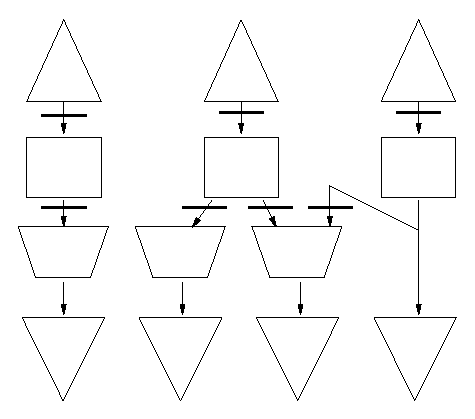
\includegraphics{figs/execute/multi-query.fig.eps}%
\end{picture}%
\setlength{\unitlength}{4144sp}%
%
\begingroup\makeatletter\ifx\SetFigFont\undefined%
\gdef\SetFigFont#1#2#3#4#5{%
  \reset@font\fontsize{#1}{#2pt}%
  \fontfamily{#3}\fontseries{#4}\fontshape{#5}%
  \selectfont}%
\fi\endgroup%
\begin{picture}(3361,2928)(34,-2098)
\end{picture}%
} &
      \scalebox{0.4}{\begin{picture}(0,0)%
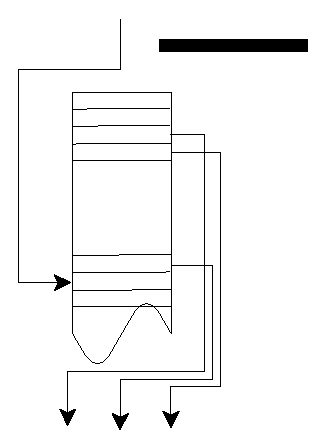
\includegraphics{figs/execute/fifo.fig.eps}%
\end{picture}%
\setlength{\unitlength}{4144sp}%
%
\begingroup\makeatletter\ifx\SetFigFont\undefined%
\gdef\SetFigFont#1#2#3#4#5{%
  \reset@font\fontsize{#1}{#2pt}%
  \fontfamily{#3}\fontseries{#4}\fontshape{#5}%
  \selectfont}%
\fi\endgroup%
\begin{picture}(2228,3153)(35,-2323)
\put(835,-457){\makebox(0,0)[b]{\smash{{\SetFigFont{12}{14.4}{\sfdefault}{\mddefault}{\updefault}{\color[rgb]{0,0,0}Pointer}%
}}}}
\put(835,-652){\makebox(0,0)[b]{\smash{{\SetFigFont{12}{14.4}{\sfdefault}{\mddefault}{\updefault}{\color[rgb]{0,0,0}Stack}%
}}}}
\end{picture}%
} &
      \scalebox{0.4}{\begin{picture}(0,0)%
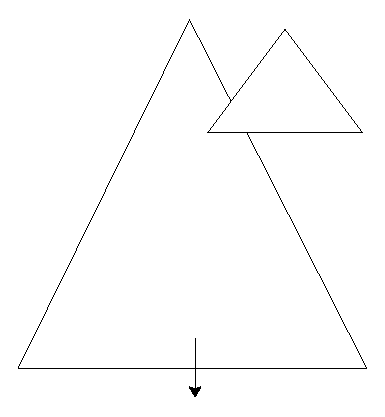
\includegraphics{figs/execute/goes.fig.eps}%
\end{picture}%
\setlength{\unitlength}{4144sp}%
%
\begingroup\makeatletter\ifx\SetFigFont\undefined%
\gdef\SetFigFont#1#2#3#4#5{%
  \reset@font\fontsize{#1}{#2pt}%
  \fontfamily{#3}\fontseries{#4}\fontshape{#5}%
  \selectfont}%
\fi\endgroup%
\begin{picture}(2679,2912)(34,-2061)
\put(676,-841){\makebox(0,0)[lb]{\smash{{\SetFigFont{10}{12.0}{\familydefault}{\mddefault}{\updefault}{\color[rgb]{0,0,0}A single \ac{GOES} }%
}}}}
\put(676,-1036){\makebox(0,0)[lb]{\smash{{\SetFigFont{10}{12.0}{\familydefault}{\mddefault}{\updefault}{\color[rgb]{0,0,0}channel is converted }%
}}}}
\put(676,-1231){\makebox(0,0)[lb]{\smash{{\SetFigFont{10}{12.0}{\familydefault}{\mddefault}{\updefault}{\color[rgb]{0,0,0}to internal format and}%
}}}}
\put(676,-1426){\makebox(0,0)[lb]{\smash{{\SetFigFont{10}{12.0}{\familydefault}{\mddefault}{\updefault}{\color[rgb]{0,0,0}input into \ac{QEP}}%
}}}}
\put(676,-646){\makebox(0,0)[lb]{\smash{{\SetFigFont{10}{12.0}{\familydefault}{\mddefault}{\updefault}{\color[rgb]{0,0,0}Direct Output for}%
}}}}
\put(2071,254){\makebox(0,0)[b]{\smash{{\SetFigFont{12}{14.4}{\familydefault}{\mddefault}{\updefault}{\color[rgb]{0,0,0}Goes}%
}}}}
\end{picture}%
} \\
      Query Graph & FIFO & GOES \\
      \scalebox{0.4}{\begin{picture}(0,0)%
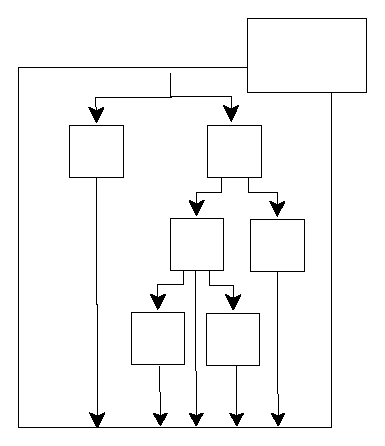
\includegraphics{figs/execute/selection.fig.eps}%
\end{picture}%
\setlength{\unitlength}{4144sp}%
%
\begingroup\makeatletter\ifx\SetFigFont\undefined%
\gdef\SetFigFont#1#2#3#4#5{%
  \reset@font\fontsize{#1}{#2pt}%
  \fontfamily{#3}\fontseries{#4}\fontshape{#5}%
  \selectfont}%
\fi\endgroup%
\begin{picture}(2678,3140)(-11,-2324)
\put(1651,-239){\makebox(0,0)[b]{\smash{{\SetFigFont{8}{9.6}{\familydefault}{\mddefault}{\updefault}{\color[rgb]{0,0,0}Q3}%
}}}}
\put(596,-244){\makebox(0,0)[b]{\smash{{\SetFigFont{8}{9.6}{\familydefault}{\mddefault}{\updefault}{\color[rgb]{0,0,0}Q1}%
}}}}
\put(1360,-952){\makebox(0,0)[b]{\smash{{\SetFigFont{8}{9.6}{\familydefault}{\mddefault}{\updefault}{\color[rgb]{0,0,0}Q2}%
}}}}
\put(1974,-959){\makebox(0,0)[b]{\smash{{\SetFigFont{8}{9.6}{\familydefault}{\mddefault}{\updefault}{\color[rgb]{0,0,0}Q6}%
}}}}
\put(1638,-1672){\makebox(0,0)[b]{\smash{{\SetFigFont{8}{9.6}{\familydefault}{\mddefault}{\updefault}{\color[rgb]{0,0,0}Q5}%
}}}}
\put(1064,-1667){\makebox(0,0)[b]{\smash{{\SetFigFont{8}{9.6}{\familydefault}{\mddefault}{\updefault}{\color[rgb]{0,0,0}Q4}%
}}}}
\put(1878,466){\makebox(0,0)[lb]{\smash{{\SetFigFont{14}{16.8}{\familydefault}{\mddefault}{\updefault}{\color[rgb]{0,0,0}$|_{\ps{X}}$}%
}}}}
\put(766,569){\makebox(0,0)[lb]{\smash{{\SetFigFont{14}{16.8}{\familydefault}{\mddefault}{\updefault}{\color[rgb]{0,0,0}\ps{X}}%
}}}}
\end{picture}%
} &
      \scalebox{0.4}{\begin{picture}(0,0)%
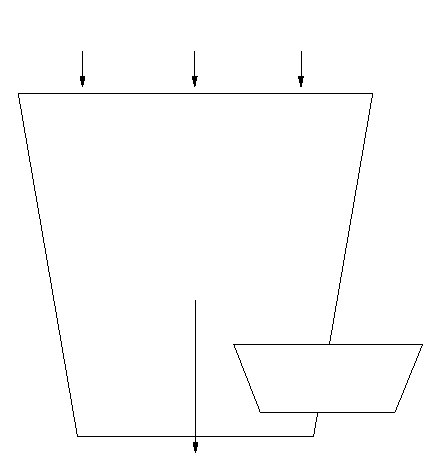
\includegraphics{figs/execute/function.fig.eps}%
\end{picture}%
\setlength{\unitlength}{4144sp}%
%
\begingroup\makeatletter\ifx\SetFigFont\undefined%
\gdef\SetFigFont#1#2#3#4#5{%
  \reset@font\fontsize{#1}{#2pt}%
  \fontfamily{#3}\fontseries{#4}\fontshape{#5}%
  \selectfont}%
\fi\endgroup%
\begin{picture}(3105,3353)(-11,-2523)
\put(361,659){\makebox(0,0)[lb]{\smash{{\SetFigFont{11}{13.2}{\familydefault}{\mddefault}{\updefault}{\color[rgb]{0,0,0}$X_1$}%
}}}}
\put(1216,659){\makebox(0,0)[lb]{\smash{{\SetFigFont{11}{13.2}{\familydefault}{\mddefault}{\updefault}{\color[rgb]{0,0,0}$X_2$}%
}}}}
\put(2026,659){\makebox(0,0)[lb]{\smash{{\SetFigFont{11}{13.2}{\familydefault}{\mddefault}{\updefault}{\color[rgb]{0,0,0}$X_3$}%
}}}}
\put(271,-106){\makebox(0,0)[lb]{\smash{{\SetFigFont{14}{16.8}{\familydefault}{\mddefault}{\updefault}{\color[rgb]{0,0,0}$f(x_1,x_2,x_3,\ldots)$}%
}}}}
\end{picture}%
} & \\
      Restriction & Induced &  \\
    \end{tabular}
\end{slide}

% \begin{slide}{Multi-output FIFOs}
%   \begin{minipage}[c]{5cm}
%     \begin{picture}(0,0)%
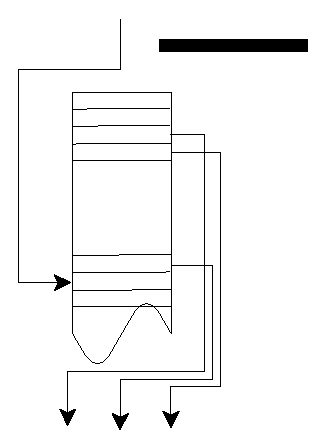
\includegraphics{figs/execute/fifo.fig.eps}%
\end{picture}%
\setlength{\unitlength}{4144sp}%
%
\begingroup\makeatletter\ifx\SetFigFont\undefined%
\gdef\SetFigFont#1#2#3#4#5{%
  \reset@font\fontsize{#1}{#2pt}%
  \fontfamily{#3}\fontseries{#4}\fontshape{#5}%
  \selectfont}%
\fi\endgroup%
\begin{picture}(2228,3153)(35,-2323)
\put(835,-457){\makebox(0,0)[b]{\smash{{\SetFigFont{12}{14.4}{\sfdefault}{\mddefault}{\updefault}{\color[rgb]{0,0,0}Pointer}%
}}}}
\put(835,-652){\makebox(0,0)[b]{\smash{{\SetFigFont{12}{14.4}{\sfdefault}{\mddefault}{\updefault}{\color[rgb]{0,0,0}Stack}%
}}}}
\end{picture}%

%   \end{minipage}
%   \begin{minipage}[c]{5cm}
%     \begin{Itemize}
%     \item Single Input
%     \item Multiple Outputs
%     \item Potentially Large
%     \item Can control via threads
%     \end{Itemize}
%   \end{minipage}
% \end{slide}

% \begin{slide}{GOES Input}
%   \begin{minipage}[c]{5cm}
%     \begin{picture}(0,0)%
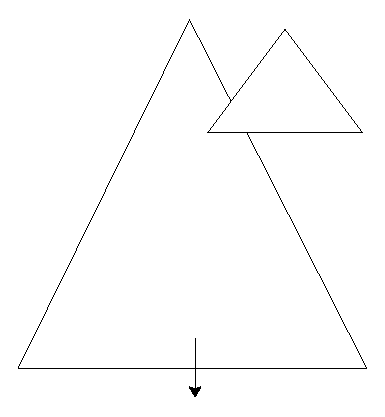
\includegraphics{figs/execute/goes.fig.eps}%
\end{picture}%
\setlength{\unitlength}{4144sp}%
%
\begingroup\makeatletter\ifx\SetFigFont\undefined%
\gdef\SetFigFont#1#2#3#4#5{%
  \reset@font\fontsize{#1}{#2pt}%
  \fontfamily{#3}\fontseries{#4}\fontshape{#5}%
  \selectfont}%
\fi\endgroup%
\begin{picture}(2679,2912)(34,-2061)
\put(676,-841){\makebox(0,0)[lb]{\smash{{\SetFigFont{10}{12.0}{\familydefault}{\mddefault}{\updefault}{\color[rgb]{0,0,0}A single \ac{GOES} }%
}}}}
\put(676,-1036){\makebox(0,0)[lb]{\smash{{\SetFigFont{10}{12.0}{\familydefault}{\mddefault}{\updefault}{\color[rgb]{0,0,0}channel is converted }%
}}}}
\put(676,-1231){\makebox(0,0)[lb]{\smash{{\SetFigFont{10}{12.0}{\familydefault}{\mddefault}{\updefault}{\color[rgb]{0,0,0}to internal format and}%
}}}}
\put(676,-1426){\makebox(0,0)[lb]{\smash{{\SetFigFont{10}{12.0}{\familydefault}{\mddefault}{\updefault}{\color[rgb]{0,0,0}input into \ac{QEP}}%
}}}}
\put(676,-646){\makebox(0,0)[lb]{\smash{{\SetFigFont{10}{12.0}{\familydefault}{\mddefault}{\updefault}{\color[rgb]{0,0,0}Direct Output for}%
}}}}
\put(2071,254){\makebox(0,0)[b]{\smash{{\SetFigFont{12}{14.4}{\familydefault}{\mddefault}{\updefault}{\color[rgb]{0,0,0}Goes}%
}}}}
\end{picture}%

%   \end{minipage}
%   \begin{minipage}[c]{5cm}
%     \begin{Itemize}
%     \item Converts Raw Input
%     \item Decodes GOES Metadata
%     \item Pushes QEP
%     \end{Itemize}
%   \end{minipage}
% \end{slide}

% \begin{slide}{Restrictions}
%   \begin{minipage}[c]{5cm}
%     \begin{picture}(0,0)%
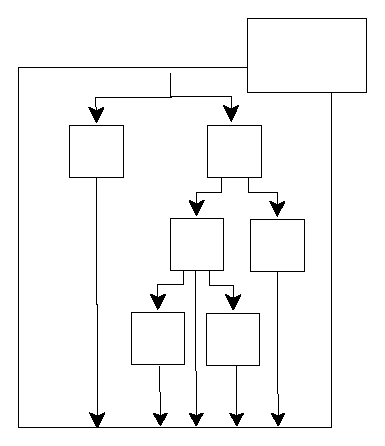
\includegraphics{figs/execute/selection.fig.eps}%
\end{picture}%
\setlength{\unitlength}{4144sp}%
%
\begingroup\makeatletter\ifx\SetFigFont\undefined%
\gdef\SetFigFont#1#2#3#4#5{%
  \reset@font\fontsize{#1}{#2pt}%
  \fontfamily{#3}\fontseries{#4}\fontshape{#5}%
  \selectfont}%
\fi\endgroup%
\begin{picture}(2678,3140)(-11,-2324)
\put(1651,-239){\makebox(0,0)[b]{\smash{{\SetFigFont{8}{9.6}{\familydefault}{\mddefault}{\updefault}{\color[rgb]{0,0,0}Q3}%
}}}}
\put(596,-244){\makebox(0,0)[b]{\smash{{\SetFigFont{8}{9.6}{\familydefault}{\mddefault}{\updefault}{\color[rgb]{0,0,0}Q1}%
}}}}
\put(1360,-952){\makebox(0,0)[b]{\smash{{\SetFigFont{8}{9.6}{\familydefault}{\mddefault}{\updefault}{\color[rgb]{0,0,0}Q2}%
}}}}
\put(1974,-959){\makebox(0,0)[b]{\smash{{\SetFigFont{8}{9.6}{\familydefault}{\mddefault}{\updefault}{\color[rgb]{0,0,0}Q6}%
}}}}
\put(1638,-1672){\makebox(0,0)[b]{\smash{{\SetFigFont{8}{9.6}{\familydefault}{\mddefault}{\updefault}{\color[rgb]{0,0,0}Q5}%
}}}}
\put(1064,-1667){\makebox(0,0)[b]{\smash{{\SetFigFont{8}{9.6}{\familydefault}{\mddefault}{\updefault}{\color[rgb]{0,0,0}Q4}%
}}}}
\put(1878,466){\makebox(0,0)[lb]{\smash{{\SetFigFont{14}{16.8}{\familydefault}{\mddefault}{\updefault}{\color[rgb]{0,0,0}$|_{\ps{X}}$}%
}}}}
\put(766,569){\makebox(0,0)[lb]{\smash{{\SetFigFont{14}{16.8}{\familydefault}{\mddefault}{\updefault}{\color[rgb]{0,0,0}\ps{X}}%
}}}}
\end{picture}%

%   \end{minipage}
%   \begin{minipage}[c]{5cm}
%     \begin{Itemize}
%     \item Single Input
%     \item Many Outputs
%     \item Has Selectivity
%     \end{Itemize}
%   \end{minipage}
% \end{slide}

% \begin{slide}{Space Saving Partitioning}
%   \centering
%   { \fontsize{4}{4}\selectfont
%     \psset{unit=0.5}
%     \begin{tabular}{cccc}
%     {  
%       \begin{FramePic}[5,5]
%         \roi[style=query](1,0)(4,3){$S$}
%         \roi[style=query](2,1)(5,4){$T$}
%       \end{FramePic}
%     } &
%     {
%       \begin{FramePic}[5,5]
%         \roI[style=frame](0,4)(5,5){$\perp$}{$x_{00}$}
        
%         \roI[style=frame](0,3)(2,4){$\perp$}{$x_{10}$}
%         \roI[style=query](2,3)(5,4){\tiny{$\{T\}$}}{$x_{11}$}
        
%         \roI[style=frame](0,2)(1,3){$\perp$}{$x_{20}$}
%         \roI[style=query](1,2)(2,3){\tiny{$\{S\}$}}{$x_{21}$}
%         \roI[style=query](2,2)(4,3){\tiny{$\{S,T\}$}}{$x_{22}$}
%         \roI[style=frame](4,2)(5,3){\tiny{$\{T\}$}}{$x_{23}$}
        
%         \roI[style=frame](0,1)(1,2){$\perp$}{$x_{30}$}
%         \roI[style=query](1,1)(2,2){\tiny{$\{S\}$}}{$x_{31}$}
%         \roI[style=query](2,1)(4,2){\tiny{$\{S,T\}$}}{$x_{32}$}
%         \roI[style=frame](4,1)(5,2){\tiny{$\{T\}$}}{$x_{33}$}
        
%         \roI[style=frame](0,0)(1,1){$\perp$}{$x_{40}$}
%         \roI[style=query](1,0)(4,1){\tiny{$\{S\}$}}{$x_{41}$}
%         \roI[style=query](4,0)(5,1){$\perp$}{$x_{42}$}
%       \end{FramePic}
%     } &
%     {
%       \begin{FramePic}[5,5]
%         \roI[style=frame](0,4)(5,5){$\perp$}{$x_{00}$}
%         \roI[style=frame](0,3)(5,4){$\perp$}{$x_{00}$}
        
%         \roI[style=frame](0,2)(1,3){$\perp$}{$x_{20}$}
%         \roI[style=query](1,2)(4,3){\tiny{$\{S\}$}}{$x_{21}$}
%         \roI[style=frame](4,2)(5,3){$\perp$}{$x_{22}$}
        
%         \roI[style=frame](0,1)(1,2){$\perp$}{$x_{30}$}
%         \roI[style=query](1,1)(4,2){\tiny{$\{S\}$}}{$x_{31}$}
%         \roI[style=frame](4,1)(5,2){$\perp$}{$x_{32}$}
        
%         \roI[style=frame](0,0)(1,1){$\perp$}{$x_{30}$}
%         \roI[style=query](1,0)(4,1){\tiny{$\{S\}$}}{$x_{31}$}
%         \roI[style=query](4,0)(5,1){$\perp$}{$x_{32}$}
%       \end{FramePic}
%     } &
%     {
%       \begin{FramePic}[5,5]
%         \roI[style=frame](0,4)(5,5){$\perp$}{$x_{00}$}
        
%         \roI[style=frame](0,3)(2,4){$\perp$}{$x_{10}$}
%         \roI[style=query](2,3)(5,4){\tiny{$\{T\}$}}{$x_{11}$}
        
%         \roI[style=frame](0,2)(2,3){$\perp$}{$x_{20}$}
%         \roI[style=frame](2,2)(5,3){\tiny{$\{T\}$}}{$x_{21}$}
        
%         \roI[style=frame](0,1)(2,2){$\perp$}{$x_{30}$}
%         \roI[style=frame](2,1)(5,2){\tiny{$\{T\}$}}{$x_{31}$}
        
%         \roI[style=frame](0,0)(5,1){$\perp$}{$x_{30}$}
%       \end{FramePic}
%     } \\
%     input &
%     multiple divisions &
%     \ps{S} output &
%     \ps{T} output \\
% \end{tabular}
% }
% \end{slide}

\begin{slide}{Row Partitioning}
  \centering
  { \psset{unit=0.25}
  \begin{tabular}{cc}
    {
      \begin{FramePic}[10,10]
        \psframe[fillstyle=solid,fillcolor=gray](0,4)(10,5)
        \psgrid[gridcolor=lightgray,subgriddiv=0,gridlabels=0,gridwidth=1pt](0,4)(10,5)
        \roi[style=query](1,1)(6,6){$S$}
        \roi[style=query](2,4)(9,8){$T$}
      \end{FramePic}} &
    {
      \begin{pspicture}(10,10)
        \uput{7pt}[u](5,6){$S:(s_n,s_x,r,i_s)$}
        \psframe[fillstyle=solid,fillcolor=gray](1,6)(6,7)
        \psgrid[gridcolor=lightgray,subgriddiv=0,gridlabels=0,gridwidth=1pt](0,6)(10,7)
        \uput{7pt}[u](5,2){$T:(t_n,t_x,r,i_t)$}
        \psframe[fillstyle=solid,fillcolor=gray](2,2)(9,3)
        \psgrid[gridcolor=lightgray,subgriddiv=0,gridlabels=0,gridwidth=1pt](0,2)(10,3)
      \end{pspicture}
    } \\
    input row & output rows \\
  \end{tabular}
}
\end{slide}

% \begin{slide}{Induced Operators}
%   \begin{minipage}[c]{5cm}
%     \begin{picture}(0,0)%
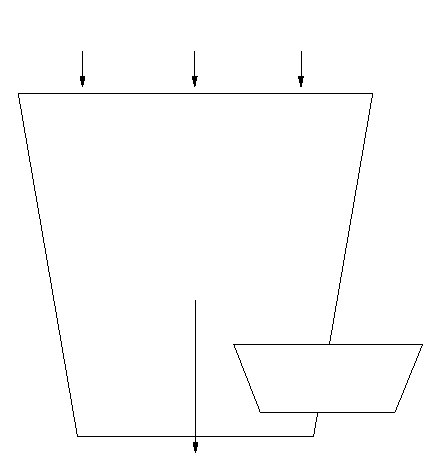
\includegraphics{figs/execute/function.fig.eps}%
\end{picture}%
\setlength{\unitlength}{4144sp}%
%
\begingroup\makeatletter\ifx\SetFigFont\undefined%
\gdef\SetFigFont#1#2#3#4#5{%
  \reset@font\fontsize{#1}{#2pt}%
  \fontfamily{#3}\fontseries{#4}\fontshape{#5}%
  \selectfont}%
\fi\endgroup%
\begin{picture}(3105,3353)(-11,-2523)
\put(361,659){\makebox(0,0)[lb]{\smash{{\SetFigFont{11}{13.2}{\familydefault}{\mddefault}{\updefault}{\color[rgb]{0,0,0}$X_1$}%
}}}}
\put(1216,659){\makebox(0,0)[lb]{\smash{{\SetFigFont{11}{13.2}{\familydefault}{\mddefault}{\updefault}{\color[rgb]{0,0,0}$X_2$}%
}}}}
\put(2026,659){\makebox(0,0)[lb]{\smash{{\SetFigFont{11}{13.2}{\familydefault}{\mddefault}{\updefault}{\color[rgb]{0,0,0}$X_3$}%
}}}}
\put(271,-106){\makebox(0,0)[lb]{\smash{{\SetFigFont{14}{16.8}{\familydefault}{\mddefault}{\updefault}{\color[rgb]{0,0,0}$f(x_1,x_2,x_3,\ldots)$}%
}}}}
\end{picture}%

%   \end{minipage}
%   \begin{minipage}[c]{5cm}
%     \begin{Itemize}
%     \item One Input
%     \item One Output
%     \item General Functions
%     \item Make Data, Expensive
%     \end{Itemize}
%   \end{minipage}
% \end{slide}

\begin{slide}{Geometric Transformations}
  \begin{Itemize}
  \item Geometric transformations impede stream flow
  \item Operator needs to minimize blocking
  \end{Itemize}
  \centering
  \scalebox{0.6}{\input{figs/geometric-transform.fig.tex}}
\end{slide}

\begin{slide}{Contributions}
  \begin{Itemize}
  \item Identified operator requirements
  \item Developed multi-output FIFO
  \item Developed shared restriction operator
  \item Will develop other operators
  \end{Itemize}
\end{slide}

% \begin{slide}{Roadmap}
%   \begin{Itemize}
%   {\tiny
%   \item Overview and Background
%   \item Models
%   \item Query Processing
%   \item Operators
%   }
%   {\blue \item The Dynamic Cascade Tree
%     \begin{itemize}
%     \item Problem Description
%     \item Description
%     \item Performance
%     \item Results
%     \end{itemize}
%   }
%   {\tiny 
%   \item Conclusions and Work Plan
%   }
%   \end{Itemize}
% \end{slide}

\begin{slide}{Roadmap - Dynamic Cascade Tree}
  {\tiny \ii Overview and Background \ii Models \ii Query Processing \ii Operators }
  \begin{Itemize}
  \item Dynamic Cascade Tree \\ {\blue Objectives / Contributions}
      \begin{Itemize}
      \item Define a restriction operator that conforms to
        requirements of image DSMSs
      \item Wider use as an index for streaming geo-spatial data
      \end{Itemize}
      {\blue Related Work}
      \begin{Itemize}
      \item Grouped filters, query index, R-tree variants, segment
        trees, grids
      \item Incremental schemes, regions of validity
      \end{Itemize}
    \end{Itemize}
  {\tiny \ii Conclusions and Work Plan }
\end{slide}

\begin{slide}[R]{Problem Description}
  Quickly direct the incoming data streams (GOES imagery) to
  the appropriate queries based on the regions of interest from the
  active user queries.
  \begin{itemize}
  \item Small in-memory index 
  \item Moving input (Stabs)
    \begin{itemize}
    \item Small number of streaming data (satellites) locations
    \item Data stream queries usually are close to one another
    \item Regular trajectory through regions
    \end{itemize}
  \item Input stream (stabs) are points or boxes
    \begin{itemize}
    \item Typically thin ($\frac{x}{y} >> 1$) boxes
    \end{itemize}
  \item High selectivity per stab (20\%)
  \item Need fast insertion and deletion of regions of interest
  \end{itemize}
\end{slide}


% DCT has [40-60] !50
\begin{slide}[R]{DCT - Simple}
\input{presentation/dct.pstex_t}
\end{slide}

% Insert +70
\begin{slide}[R]{DCT - Insert New Region}
\input{presentation/dct-insert.pstex_t}
\end{slide}

% % Delete - 60 
% \begin{slide}[R]{DCT - Delete Region}
% \input{presentation/dct-delete.pstex_t}
% \end{slide}

% % MoveY -40 +35
% \begin{slide}[R]{DCT - Move \Y Direction}
% \input{presentation/dct-moveY.pstex_t}
% \end{slide}

% Move X +32 
\begin{slide}[R]{DCT - New Query}
\input{presentation/dct-moveX.pstex_t}
\end{slide}

% % -32 -35 -40 +110 
% \begin{slide}[R]{DCT - Box}
% \input{presentation/dct-box.pstex_t}
% \end{slide}

% % +25 +105 -110
% \begin{slide}[R]{DCT - Box Move}
% \input{presentation/dct-box-move.pstex_t}
% \end{slide}

\begin{slide}{DCT - Boxes}
  \centering
  \scalebox{0.8}{\begin{picture}(0,0)%
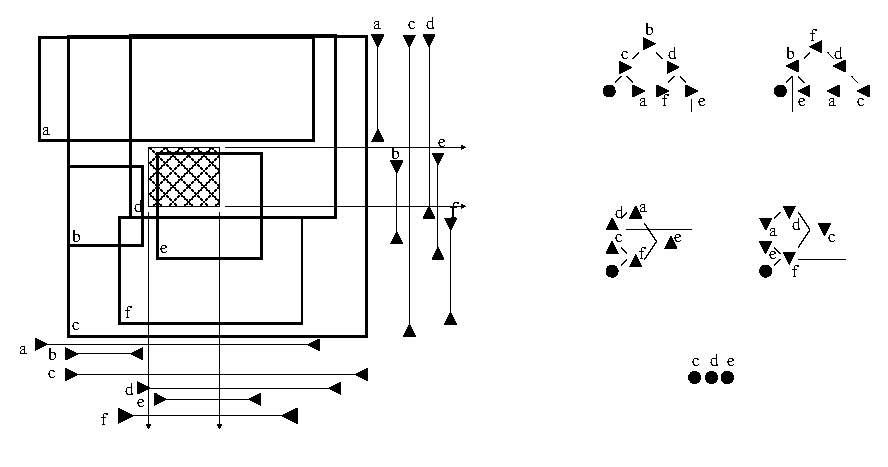
\includegraphics{figs/dct.fig.eps}%
\end{picture}%
\setlength{\unitlength}{4144sp}%
%
\begingroup\makeatletter\ifx\SetFigFont\undefined%
\gdef\SetFigFont#1#2#3#4#5{%
  \reset@font\fontsize{#1}{#2pt}%
  \fontfamily{#3}\fontseries{#4}\fontshape{#5}%
  \selectfont}%
\fi\endgroup%
\begin{picture}(6507,3300)(76,-2506)
\put(991,-2491){\makebox(0,0)[lb]{\smash{{\SetFigFont{8}{9.6}{\familydefault}{\mddefault}{\updefault}{\color[rgb]{0,0,0}\wxn}%
}}}}
\put(1531,-2491){\makebox(0,0)[lb]{\smash{{\SetFigFont{8}{9.6}{\familydefault}{\mddefault}{\updefault}{\color[rgb]{0,0,0}\wxx}%
}}}}
\put(3601,-196){\makebox(0,0)[lb]{\smash{{\SetFigFont{8}{9.6}{\familydefault}{\mddefault}{\updefault}{\color[rgb]{0,0,0}\wyx}%
}}}}
\put(3601,-691){\makebox(0,0)[lb]{\smash{{\SetFigFont{8}{9.6}{\familydefault}{\mddefault}{\updefault}{\color[rgb]{0,0,0}\wyn}%
}}}}
\put(4141,-1456){\makebox(0,0)[lb]{\smash{{\SetFigFont{9}{10.8}{\rmdefault}{\mddefault}{\updefault}{\color[rgb]{0,0,0}$y$-dim trees include CQ regions that overlap}%
}}}}
\put(5131,-1636){\makebox(0,0)[lb]{\smash{{\SetFigFont{9}{10.8}{\rmdefault}{\mddefault}{\updefault}{\color[rgb]{0,0,0}in $x$ dimension.}%
}}}}
\put(4681,-241){\makebox(0,0)[lb]{\smash{{\SetFigFont{9}{10.8}{\rmdefault}{\mddefault}{\updefault}{\color[rgb]{0,0,0}$x$-dim trees include all CQ regions}%
}}}}
\put(4321,-2221){\makebox(0,0)[lb]{\smash{{\SetFigFont{9}{10.8}{\rmdefault}{\mddefault}{\updefault}{\color[rgb]{0,0,0}\A\ includes regions overlapping in $x$ and $y$}%
}}}}
\put(5266,-871){\makebox(0,0)[lb]{\smash{{\SetFigFont{9}{10.8}{\rmdefault}{\mddefault}{\updefault}{\color[rgb]{0,0,0}\wyx}%
}}}}
\put(5266,-691){\makebox(0,0)[lb]{\smash{{\SetFigFont{9}{10.8}{\rmdefault}{\mddefault}{\updefault}{\color[rgb]{0,0,0}\Yn}%
}}}}
\put(6436,-1096){\makebox(0,0)[lb]{\smash{{\SetFigFont{9}{10.8}{\rmdefault}{\mddefault}{\updefault}{\color[rgb]{0,0,0}\wyn}%
}}}}
\put(6391,-691){\makebox(0,0)[lb]{\smash{{\SetFigFont{9}{10.8}{\rmdefault}{\mddefault}{\updefault}{\color[rgb]{0,0,0}\Yx}%
}}}}
\put(5131,-61){\makebox(0,0)[lb]{\smash{{\SetFigFont{9}{10.8}{\rmdefault}{\mddefault}{\updefault}{\color[rgb]{0,0,0}\wxx}%
}}}}
\put(5311,524){\makebox(0,0)[lb]{\smash{{\SetFigFont{9}{10.8}{\rmdefault}{\mddefault}{\updefault}{\color[rgb]{0,0,0}\Xn}%
}}}}
\put(6481,569){\makebox(0,0)[lb]{\smash{{\SetFigFont{9}{10.8}{\rmdefault}{\mddefault}{\updefault}{\color[rgb]{0,0,0}\Xx}%
}}}}
\put(5896,-61){\makebox(0,0)[lb]{\smash{{\SetFigFont{9}{10.8}{\rmdefault}{\mddefault}{\updefault}{\color[rgb]{0,0,0}\wxn}%
}}}}
\put(5896,-1996){\makebox(0,0)[lb]{\smash{{\SetFigFont{9}{10.8}{\rmdefault}{\mddefault}{\updefault}{\color[rgb]{0,0,0}\A}%
}}}}
\end{picture}%
}
\end{slide}

\begin{slide}[R]{Performance}
  \begin{itemize}    
  \item Small size $\Theta(n)$
  \item Fast insertions/deletions of regions $O(\lg{n})$ 
  \item Query cost from $\Omega(k)$ to $O(n\lg{n}+k)$
%%     \begin{itemize}
%%     \item  ``Rule of Thumb'' $\lg{n}$ crossings per stab $\lg^2{n} + k$
%%     \end{itemize}
  \item Data stream trajectory path
    \begin{itemize}
    \item Better to move in dimension(s) of lower cascade(s), which
      limits the number of potential regions, and avoids more costly
      insertions
    \item Total insertion of $O(n\lg{n})$ for monotonic paths
    \end{itemize}
%%   \item Independent of other parameters (except for $k$)
%%     \begin{itemize}
%%     \item Size /Shape of indexed regions
%%     \item Size / Shape of query region 
%%     \end{itemize}
  \end{itemize}
  \hfill $n$ is number of regions \\
  \hfill $k$ is number of results 
\end{slide}

\begin{slide}[R]{DCT Results - Random Input}
  \begin{itemize}
  \item R*-tree: \emph{Spatial Index Library}, UC Riverside
  \item DCT: \emph{Spatial Index Library}, \emph{Standard Template Library}
    \begin{itemize}
    \item 600 lines of code
    \end{itemize}
  \end{itemize}

  \begin{minipage}[c]{5cm}
    \centering
    \vspace{0pt}
    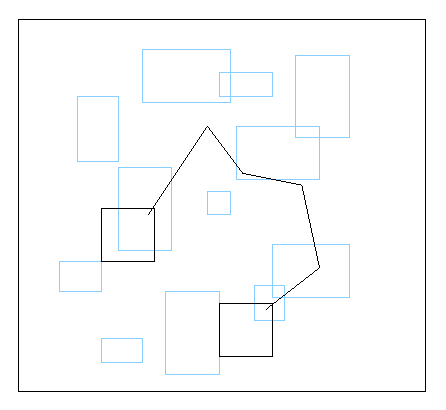
\includegraphics[width=3cm]{figs/random_tests.eps}%
  \end{minipage}
  \begin{minipage}[c]{5cm}
    \centering
    \begin{tabular}[t]{|cl|}
      \multicolumn{2}{c}{Region Parameters} \\
      \hline
      Area & 0.1-10 [\%] \\
      Aspect & 0.7-1.4 \\
      \hline
    \end{tabular}
    
    \begin{tabular}[t]{|cl|}
      \multicolumn{2}{c}{Query Parameters} \\
      \hline
      Area & 1 [\%]\\
      Aspect & 1 \\
      Distance & 1 [\%] \\
      \hline
    \end{tabular}
  \end{minipage}

\vspace{.5cm}
 \tiny 1.6 GHz Pentium M; 1MB L2; 512MB; \emph{IBM Thinkpad T40p}
 \end{slide}

%% \begin{slide}[R]{Results - Random Input}
%% \input{random_tests.pstex_t}
%% \end{slide}

\begin{slide}[R]{Inter-Query Distance}
  \centering
  \scalebox{1.3}{
    \fontsize{8}{8}\selectfont%
    %GNUPLOT: LaTeX picture with Postscript
\begin{picture}(0,0)%
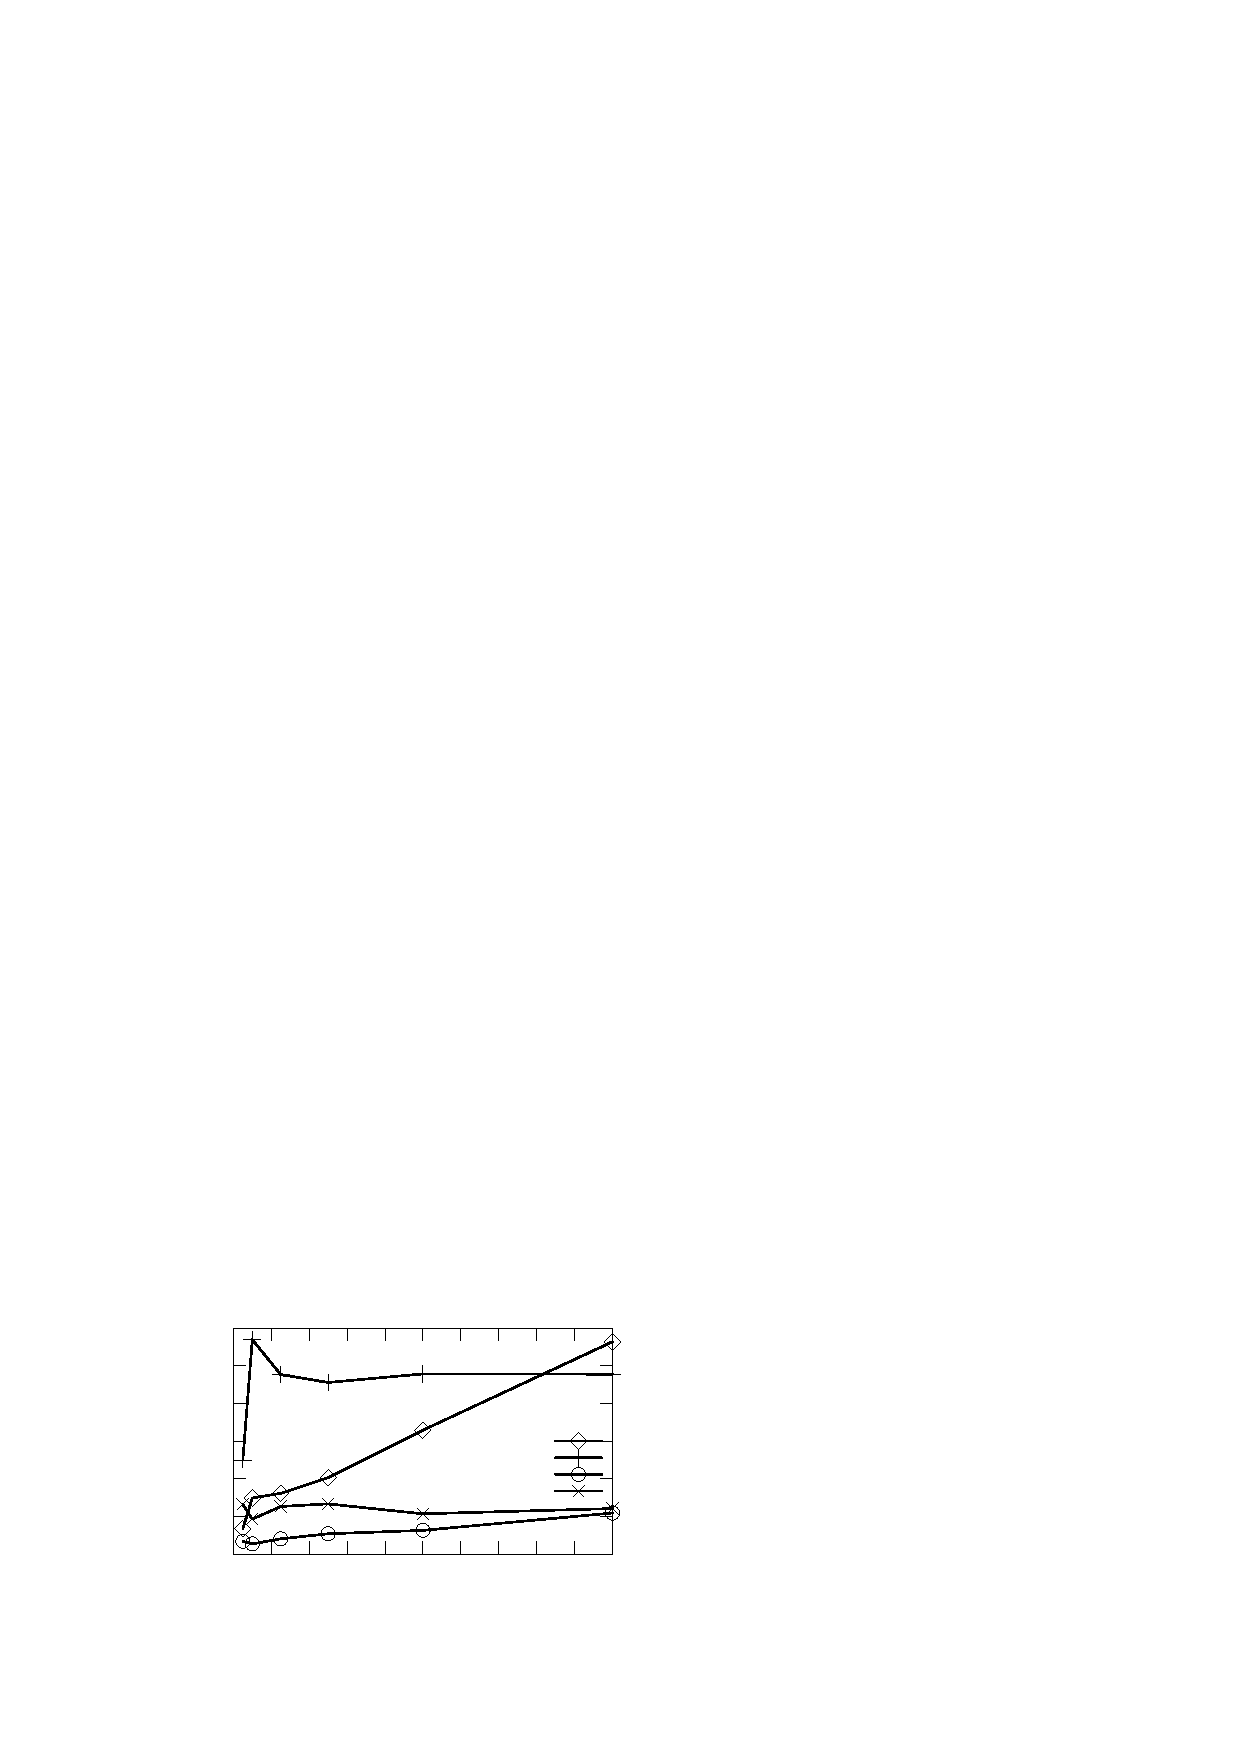
\includegraphics{dis}%
\end{picture}%
\begingroup
\setlength{\unitlength}{0.0200bp}%
\begin{picture}(11699,7019)(0,0)%
\put(1800,1200){\makebox(0,0)[r]{\strut{} 0}}%
\put(1800,2103){\makebox(0,0)[r]{\strut{} 1000}}%
\put(1800,3007){\makebox(0,0)[r]{\strut{} 2000}}%
\put(1800,3910){\makebox(0,0)[r]{\strut{} 3000}}%
\put(1800,4813){\makebox(0,0)[r]{\strut{} 4000}}%
\put(1800,5717){\makebox(0,0)[r]{\strut{} 5000}}%
\put(1800,6620){\makebox(0,0)[r]{\strut{} 6000}}%
\put(2000,800){\makebox(0,0){\strut{} 0}}%
\put(2910,800){\makebox(0,0){\strut{} 0.2}}%
\put(3820,800){\makebox(0,0){\strut{} 0.4}}%
\put(4730,800){\makebox(0,0){\strut{} 0.6}}%
\put(5640,800){\makebox(0,0){\strut{} 0.8}}%
\put(6550,800){\makebox(0,0){\strut{} 1}}%
\put(7460,800){\makebox(0,0){\strut{} 1.2}}%
\put(8370,800){\makebox(0,0){\strut{} 1.4}}%
\put(9280,800){\makebox(0,0){\strut{} 1.6}}%
\put(10190,800){\makebox(0,0){\strut{} 1.8}}%
\put(11100,800){\makebox(0,0){\strut{} 2}}%
\put(400,3910){\rotatebox{90}{\makebox(0,0){Time [$\mu s$]}}}%
\put(6550,200){\makebox(0,0){Distance Moved [\%]}}%
\put(9535,3910){\makebox(0,0)[r]{\strut{}DCT-16K}}%
\put(9535,3510){\makebox(0,0)[r]{\strut{}RTREE-16K}}%
\put(9535,3110){\makebox(0,0)[r]{\strut{}DCT-4K}}%
\put(9535,2710){\makebox(0,0)[r]{\strut{}RTREE-4K}}%
\end{picture}%
\endgroup
\endinput

  }
\end{slide}

\begin{slide}[R]{Query Area Size}
  \centering
  \scalebox{1.3}{
  \fontsize{8}{8}\selectfont%
  %GNUPLOT: LaTeX picture with Postscript
\begin{picture}(0,0)%
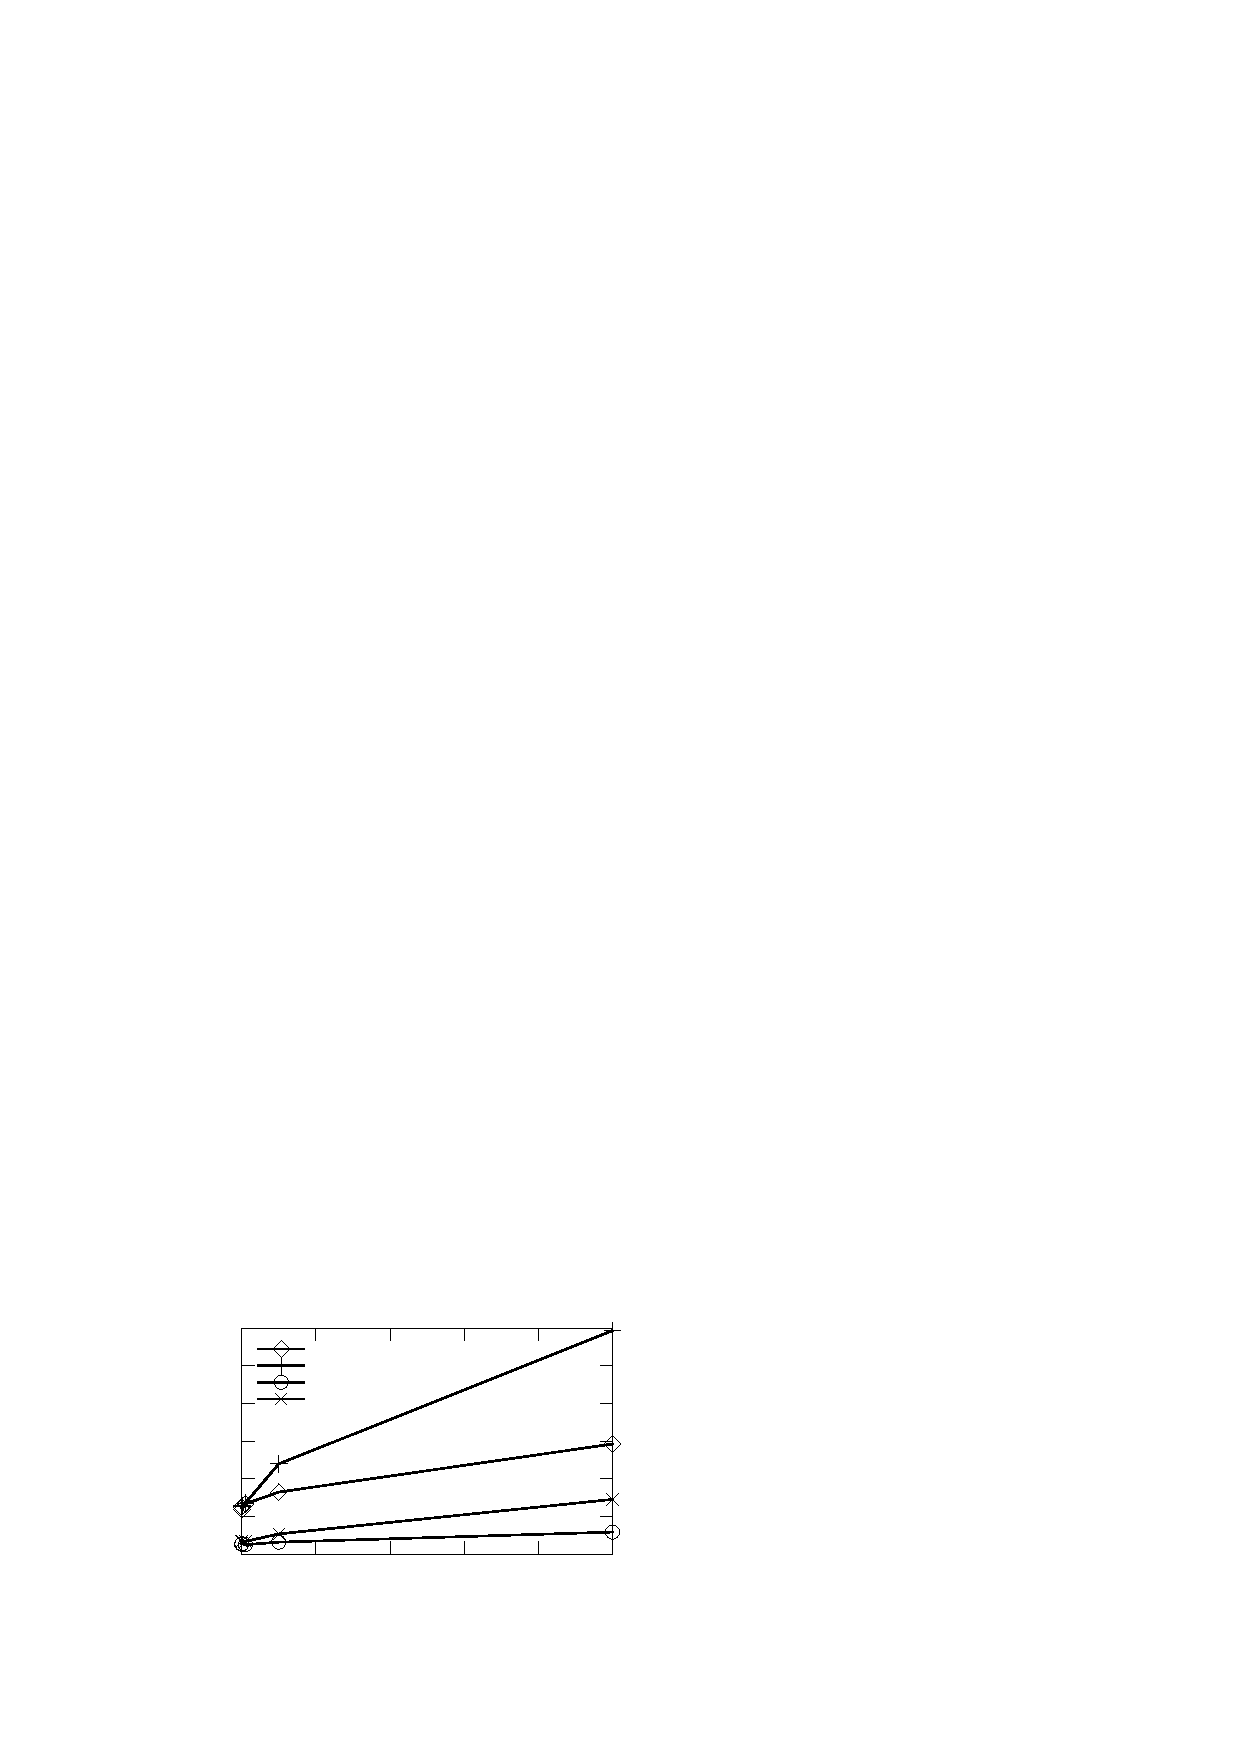
\includegraphics{stab_area}%
\end{picture}%
\begingroup
\setlength{\unitlength}{0.0200bp}%
\begin{picture}(11699,7019)(0,0)%
\put(2000,1200){\makebox(0,0)[r]{\strut{} 0}}%
\put(2000,2103){\makebox(0,0)[r]{\strut{} 2000}}%
\put(2000,3007){\makebox(0,0)[r]{\strut{} 4000}}%
\put(2000,3910){\makebox(0,0)[r]{\strut{} 6000}}%
\put(2000,4813){\makebox(0,0)[r]{\strut{} 8000}}%
\put(2000,5717){\makebox(0,0)[r]{\strut{} 10000}}%
\put(2000,6620){\makebox(0,0)[r]{\strut{} 12000}}%
\put(2200,800){\makebox(0,0){\strut{} 0}}%
\put(3980,800){\makebox(0,0){\strut{} 2}}%
\put(5760,800){\makebox(0,0){\strut{} 4}}%
\put(7540,800){\makebox(0,0){\strut{} 6}}%
\put(9320,800){\makebox(0,0){\strut{} 8}}%
\put(11100,800){\makebox(0,0){\strut{} 10}}%
\put(400,3910){\rotatebox{90}{\makebox(0,0){Time [$\mu s$]}}}%
\put(6650,200){\makebox(0,0){Window Query Area [\%]}}%
\put(3900,6120){\makebox(0,0)[l]{\strut{}DCT-16K}}%
\put(3900,5720){\makebox(0,0)[l]{\strut{}RTREE-16K}}%
\put(3900,5320){\makebox(0,0)[l]{\strut{}DCT-4K}}%
\put(3900,4920){\makebox(0,0)[l]{\strut{}RTREE-4K}}%
\end{picture}%
\endgroup
\endinput

  }
\end{slide}

\begin{slide}[R]{Query Box Aspect}
  \centering
  \scalebox{1.3}{
  \fontsize{8}{8}\selectfont%
  %GNUPLOT: LaTeX picture with Postscript
\begin{picture}(0,0)%
\includegraphics{stab_aspect}%
\end{picture}%
\begingroup
\setlength{\unitlength}{0.0200bp}%
\begin{picture}(11699,7019)(0,0)%
\put(1800,1200){\makebox(0,0)[r]{\strut{} 0}}%
\put(1800,1877){\makebox(0,0)[r]{\strut{} 1000}}%
\put(1800,2555){\makebox(0,0)[r]{\strut{} 2000}}%
\put(1800,3232){\makebox(0,0)[r]{\strut{} 3000}}%
\put(1800,3910){\makebox(0,0)[r]{\strut{} 4000}}%
\put(1800,4587){\makebox(0,0)[r]{\strut{} 5000}}%
\put(1800,5265){\makebox(0,0)[r]{\strut{} 6000}}%
\put(1800,5942){\makebox(0,0)[r]{\strut{} 7000}}%
\put(1800,6620){\makebox(0,0)[r]{\strut{} 8000}}%
\put(2000,800){\makebox(0,0){\strut{} 0}}%
\put(2910,800){\makebox(0,0){\strut{} 5}}%
\put(3820,800){\makebox(0,0){\strut{} 10}}%
\put(4730,800){\makebox(0,0){\strut{} 15}}%
\put(5640,800){\makebox(0,0){\strut{} 20}}%
\put(6550,800){\makebox(0,0){\strut{} 25}}%
\put(7460,800){\makebox(0,0){\strut{} 30}}%
\put(8370,800){\makebox(0,0){\strut{} 35}}%
\put(9280,800){\makebox(0,0){\strut{} 40}}%
\put(10190,800){\makebox(0,0){\strut{} 45}}%
\put(11100,800){\makebox(0,0){\strut{} 50}}%
\put(400,3910){\rotatebox{90}{\makebox(0,0){Time [$\mu s$]}}}%
\put(6550,200){\makebox(0,0){Window Query Aspect [$\frac{x}{y}$]}}%
\put(3700,6120){\makebox(0,0)[l]{\strut{}DCT-16K}}%
\put(3700,5720){\makebox(0,0)[l]{\strut{}RTREE-16K}}%
\put(3700,5320){\makebox(0,0)[l]{\strut{}DCT-4K}}%
\put(3700,4920){\makebox(0,0)[l]{\strut{}RTREE-4K}}%
\end{picture}%
\endgroup
\endinput

  }
\end{slide}

\begin{slide}[R]{Query Trajectory}
  \centering
  \scalebox{1.3}{
  \fontsize{8}{8}\selectfont%
  %GNUPLOT: LaTeX picture with Postscript
\begin{picture}(0,0)%
\includegraphics{dir}%
\end{picture}%
\begingroup
\setlength{\unitlength}{0.0200bp}%
\begin{picture}(11699,7019)(0,0)%
\put(1800,1200){\makebox(0,0)[r]{\strut{} 0}}%
\put(1800,2103){\makebox(0,0)[r]{\strut{} 1000}}%
\put(1800,3007){\makebox(0,0)[r]{\strut{} 2000}}%
\put(1800,3910){\makebox(0,0)[r]{\strut{} 3000}}%
\put(1800,4813){\makebox(0,0)[r]{\strut{} 4000}}%
\put(1800,5717){\makebox(0,0)[r]{\strut{} 5000}}%
\put(1800,6620){\makebox(0,0)[r]{\strut{} 6000}}%
\put(2000,800){\makebox(0,0){\strut{} 0}}%
\put(3011,800){\makebox(0,0){\strut{} 10}}%
\put(4022,800){\makebox(0,0){\strut{} 20}}%
\put(5033,800){\makebox(0,0){\strut{} 30}}%
\put(6044,800){\makebox(0,0){\strut{} 40}}%
\put(7056,800){\makebox(0,0){\strut{} 50}}%
\put(8067,800){\makebox(0,0){\strut{} 60}}%
\put(9078,800){\makebox(0,0){\strut{} 70}}%
\put(10089,800){\makebox(0,0){\strut{} 80}}%
\put(11100,800){\makebox(0,0){\strut{} 90}}%
\put(400,3910){\rotatebox{90}{\makebox(0,0){Time [$\mu s$]}}}%
\put(6550,200){\makebox(0,0){Trajectory Direction [deg]}}%
\put(9400,6120){\makebox(0,0)[r]{\strut{}DCT-16K}}%
\put(9400,5720){\makebox(0,0)[r]{\strut{}RTREE-16K}}%
\put(9400,5320){\makebox(0,0)[r]{\strut{}DCT-4K}}%
\put(9400,4920){\makebox(0,0)[r]{\strut{}RTREE-4K}}%
\end{picture}%
\endgroup
\endinput

  }
\end{slide}

\begin{slide}[R]{Region Area Size}
  \centering
  \scalebox{1.3}{
  \fontsize{8}{8}\selectfont%
  %GNUPLOT: LaTeX picture with Postscript
\begin{picture}(0,0)%
\includegraphics{area}%
\end{picture}%
\begingroup
\setlength{\unitlength}{0.0200bp}%
\begin{picture}(11699,7019)(0,0)%
\put(2000,1200){\makebox(0,0)[r]{\strut{} 0}}%
\put(2000,1877){\makebox(0,0)[r]{\strut{} 2000}}%
\put(2000,2555){\makebox(0,0)[r]{\strut{} 4000}}%
\put(2000,3232){\makebox(0,0)[r]{\strut{} 6000}}%
\put(2000,3910){\makebox(0,0)[r]{\strut{} 8000}}%
\put(2000,4587){\makebox(0,0)[r]{\strut{} 10000}}%
\put(2000,5265){\makebox(0,0)[r]{\strut{} 12000}}%
\put(2000,5942){\makebox(0,0)[r]{\strut{} 14000}}%
\put(2000,6620){\makebox(0,0)[r]{\strut{} 16000}}%
\put(2200,800){\makebox(0,0){\strut{} 0}}%
\put(3980,800){\makebox(0,0){\strut{} 5}}%
\put(5760,800){\makebox(0,0){\strut{} 10}}%
\put(7540,800){\makebox(0,0){\strut{} 15}}%
\put(9320,800){\makebox(0,0){\strut{} 20}}%
\put(11100,800){\makebox(0,0){\strut{} 25}}%
\put(400,3910){\rotatebox{90}{\makebox(0,0){Time [$\mu s$]}}}%
\put(6650,200){\makebox(0,0){Input Area [\%]}}%
\put(3900,6120){\makebox(0,0)[l]{\strut{}DCT-16K}}%
\put(3900,5720){\makebox(0,0)[l]{\strut{}RTREE-16K}}%
\put(3900,5320){\makebox(0,0)[l]{\strut{}DCT-4K}}%
\put(3900,4920){\makebox(0,0)[l]{\strut{}RTREE-4K}}%
\end{picture}%
\endgroup
\endinput

  }
\end{slide}


\begin{slide}[R]{Performance - GOES Example}
  \begin{minipage}[c]{6cm}
    \begin{itemize}
    \item 5000 regions
      \begin{itemize}
      \item 6 Hot spots (eg. North America) 
      \item Some random regions
      \end{itemize}
    \item 10000 stabbing queries
    \item Results
      \begin{itemize}
      \item \emph{R*TREE:} 48 [secs]
      \item \emph{DCT:} 9 [secs]
        \begin{itemize}
        \item 0.88 $\Omega(1)$ to $O(n\lg{n})$
        \item 8    $O(k)$
        \end{itemize}
      \end{itemize}
    \end{itemize}
%%    \begin{tabular}{cl}
%%       \multicolumn{2}{c}{Contributions} \\
%%       \hline
%%       $30\%$ & North America \\           
%%       $15\%$ & Western Seaboard \\        
%%       $15\%$ & Northern Hemisphere \\     
%%       $15\%$ & Hemisphere          \\     
%%       $9\%$  & CA                  \\    
%%       $9\%$ & Mexico              \\    
%%       $2\%$ & Random (1000x1000)  \\    
%%       $5\%$ & Random (6000x4000)       \\
%%       \hline  
%%     \end{tabular}
  \end{minipage}
   \begin{minipage}[c]{5cm}
    \includegraphics[width=6cm]{presentation/performance-goes.fig.eps}
    \par
    \begin{tabular}[b]{|cl|}
      \multicolumn{2}{c}{Region Variations} \\
      \hline
      Area & 0.8-1.2 \\
      Aspect & $\pm 10\%$ \\
      Center & $\pm 10\%$ \\ 
      \hline
    \end{tabular}
  \end{minipage}
\end{slide}

\begin{slide}{DCT - Temporal Dimension}
  \centering
  \scalebox{0.8}{\begin{picture}(0,0)%
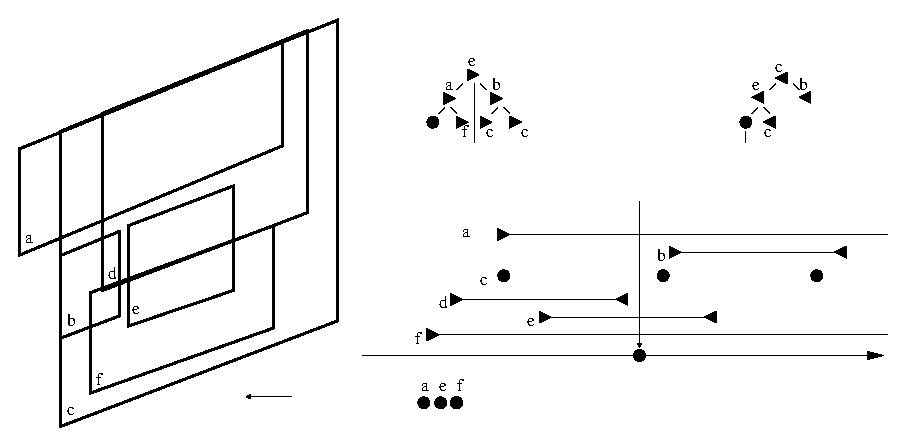
\includegraphics{figs/temporal.fig.eps}%
\end{picture}%
\setlength{\unitlength}{4144sp}%
%
\begingroup\makeatletter\ifx\SetFigFont\undefined%
\gdef\SetFigFont#1#2#3#4#5{%
  \reset@font\fontsize{#1}{#2pt}%
  \fontfamily{#3}\fontseries{#4}\fontshape{#5}%
  \selectfont}%
\fi\endgroup%
\begin{picture}(6649,3140)(69,-2288)
\put(4276,-1996){\makebox(0,0)[lb]{\smash{{\SetFigFont{10}{12.0}{\rmdefault}{\mddefault}{\updefault}{\color[rgb]{0,0,0}Time}%
}}}}
\put(2251,-2086){\makebox(0,0)[lb]{\smash{{\SetFigFont{8}{9.6}{\familydefault}{\mddefault}{\updefault}{\color[rgb]{0,0,0}Cascade to $x$}%
}}}}
\put(4726,-511){\makebox(0,0)[lb]{\smash{{\SetFigFont{8}{9.6}{\familydefault}{\mddefault}{\updefault}{\color[rgb]{0,0,0}\wt}%
}}}}
\put(6211,389){\makebox(0,0)[lb]{\smash{{\SetFigFont{11}{13.2}{\familydefault}{\mddefault}{\updefault}{\color[rgb]{0,0,0}\Tx}%
}}}}
\put(5536,-241){\makebox(0,0)[lb]{\smash{{\SetFigFont{8}{9.6}{\familydefault}{\mddefault}{\updefault}{\color[rgb]{0,0,0}\wt}%
}}}}
\put(3961,344){\makebox(0,0)[lb]{\smash{{\SetFigFont{11}{13.2}{\familydefault}{\mddefault}{\updefault}{\color[rgb]{0,0,0}\Tn}%
}}}}
\put(3466,-241){\makebox(0,0)[lb]{\smash{{\SetFigFont{8}{9.6}{\familydefault}{\mddefault}{\updefault}{\color[rgb]{0,0,0}\wt}%
}}}}
\end{picture}%
}
\end{slide}

\begin{slide}{Contributions}
  \begin{Itemize}
  \item Developed multi-output restriction operator    
  \item Showed DCT can be efficient index for general streaming geo-data
  \item Described when DCT is effective and useful
  \item Validated DCT with experimental results
  \end{Itemize}
\end{slide}

\begin{slide}{Roadmap}
  \begin{Itemize}
    {\tiny
    \item Overview and Background
    \item Models
    \item Query Processing
    \item Operators
    \item The Dynamic Cascade Tree
      }
  {\blue \item Conclusions and Work Plan}
  \end{Itemize}
\end{slide}

\begin{slide}[R]{Conclusions and Future Work}
  \begin{minipage}[t]{5.5cm}
    \raggedright
    \begin{Itemize}
    \item Architecture for remotely sensed imagery streams
      \begin{Itemize}
      \item Queries
      \item Optimizations
      \item Executions
      \end{Itemize}
    \item Restriction operator
      \begin{Itemize}
      \item Dynamic cascade tree DCT
      \item Works well for data like GOES
      \end{Itemize}
    \end{Itemize}
  \end{minipage}
  \begin{minipage}[t]{5.5cm}
    \raggedright
    \begin{Itemize}
    \item Multi-query optimizer
      \begin{Itemize}
      \item Rewrites
      \item Execution plans
      \end{Itemize}
    \item Finish operators
      \begin{Itemize}
      \item Spatial transforms
      \item Neighborhoods
      \end{Itemize}
    \item Contribute to WMS server application
    \end{Itemize}
  \end{minipage}

  \vspace*{0.5cm}

{\tiny The \emph{GeoStreams} project is supported by the NSF grant IIS-0326517}
\end{slide}

\begin{slide}{Work Plan}
  \centering
  \scalebox{0.7}{
    \begin{tabular}{c|c|l}
    Start & End & Description \\
    \hline \hline
    \multicolumn{3}{c}{Application Development} \\
    \hline
    2005-08 & 2005-11 & Complete WMS server, selection only \\
    2005-08 & 2005-09 & Complete Operator - FIFO \\
    2005-09 & 2005-10 & Complete Operator - Induced Operation \\
    2005-09 & 2006-01 & Complete Operator - Spatial Transform \\
    2006-01 & 2006-05 & Complete Operator - Neighborhoods \\
    2006-05 & 2006-09 & Complete WMS server, full service \\
    2006-06 & 2006-10 & Investigate other services \\
    \hline
    \multicolumn{3}{c}{Query Optimizations} \\    
    \hline
    2005-08 & 2005-12 & Develop graph rewriting strategies \\
    2006-01 & 2006-04 & Measure optimization performance \\
    2006-01 & 2006-09 & Implement optimizer in \ac{dsms} \\
    2006-10 & 2006-12 & Complete thesis 
  \end{tabular}
  }
\end{slide}

\begin{slide}{Geo-spatial Databases}
  \begin{Itemize}
  \item Spatial Extent
  \item Entity-Based vs. Field-Based
  \item Half-plane constraints
  \item Tessellations
  \end{Itemize}
\end{slide}

\begin{slide}{Data Stream Management Systems}
  \begin{Itemize}
  \item Data arrives in continuous data streams
  \item Research
    \begin{Itemize}
    \item Formalisms
    \item Adaptivity, operator scheduling, load shedding
    \end{Itemize}
  \item Spatio-temporal
    \begin{Itemize}
    \item Queries over moving objects
    \end{Itemize}
  \end{Itemize}
\end{slide}

\begin{slide}{Meteorological Remote Sensing}
  \centering
  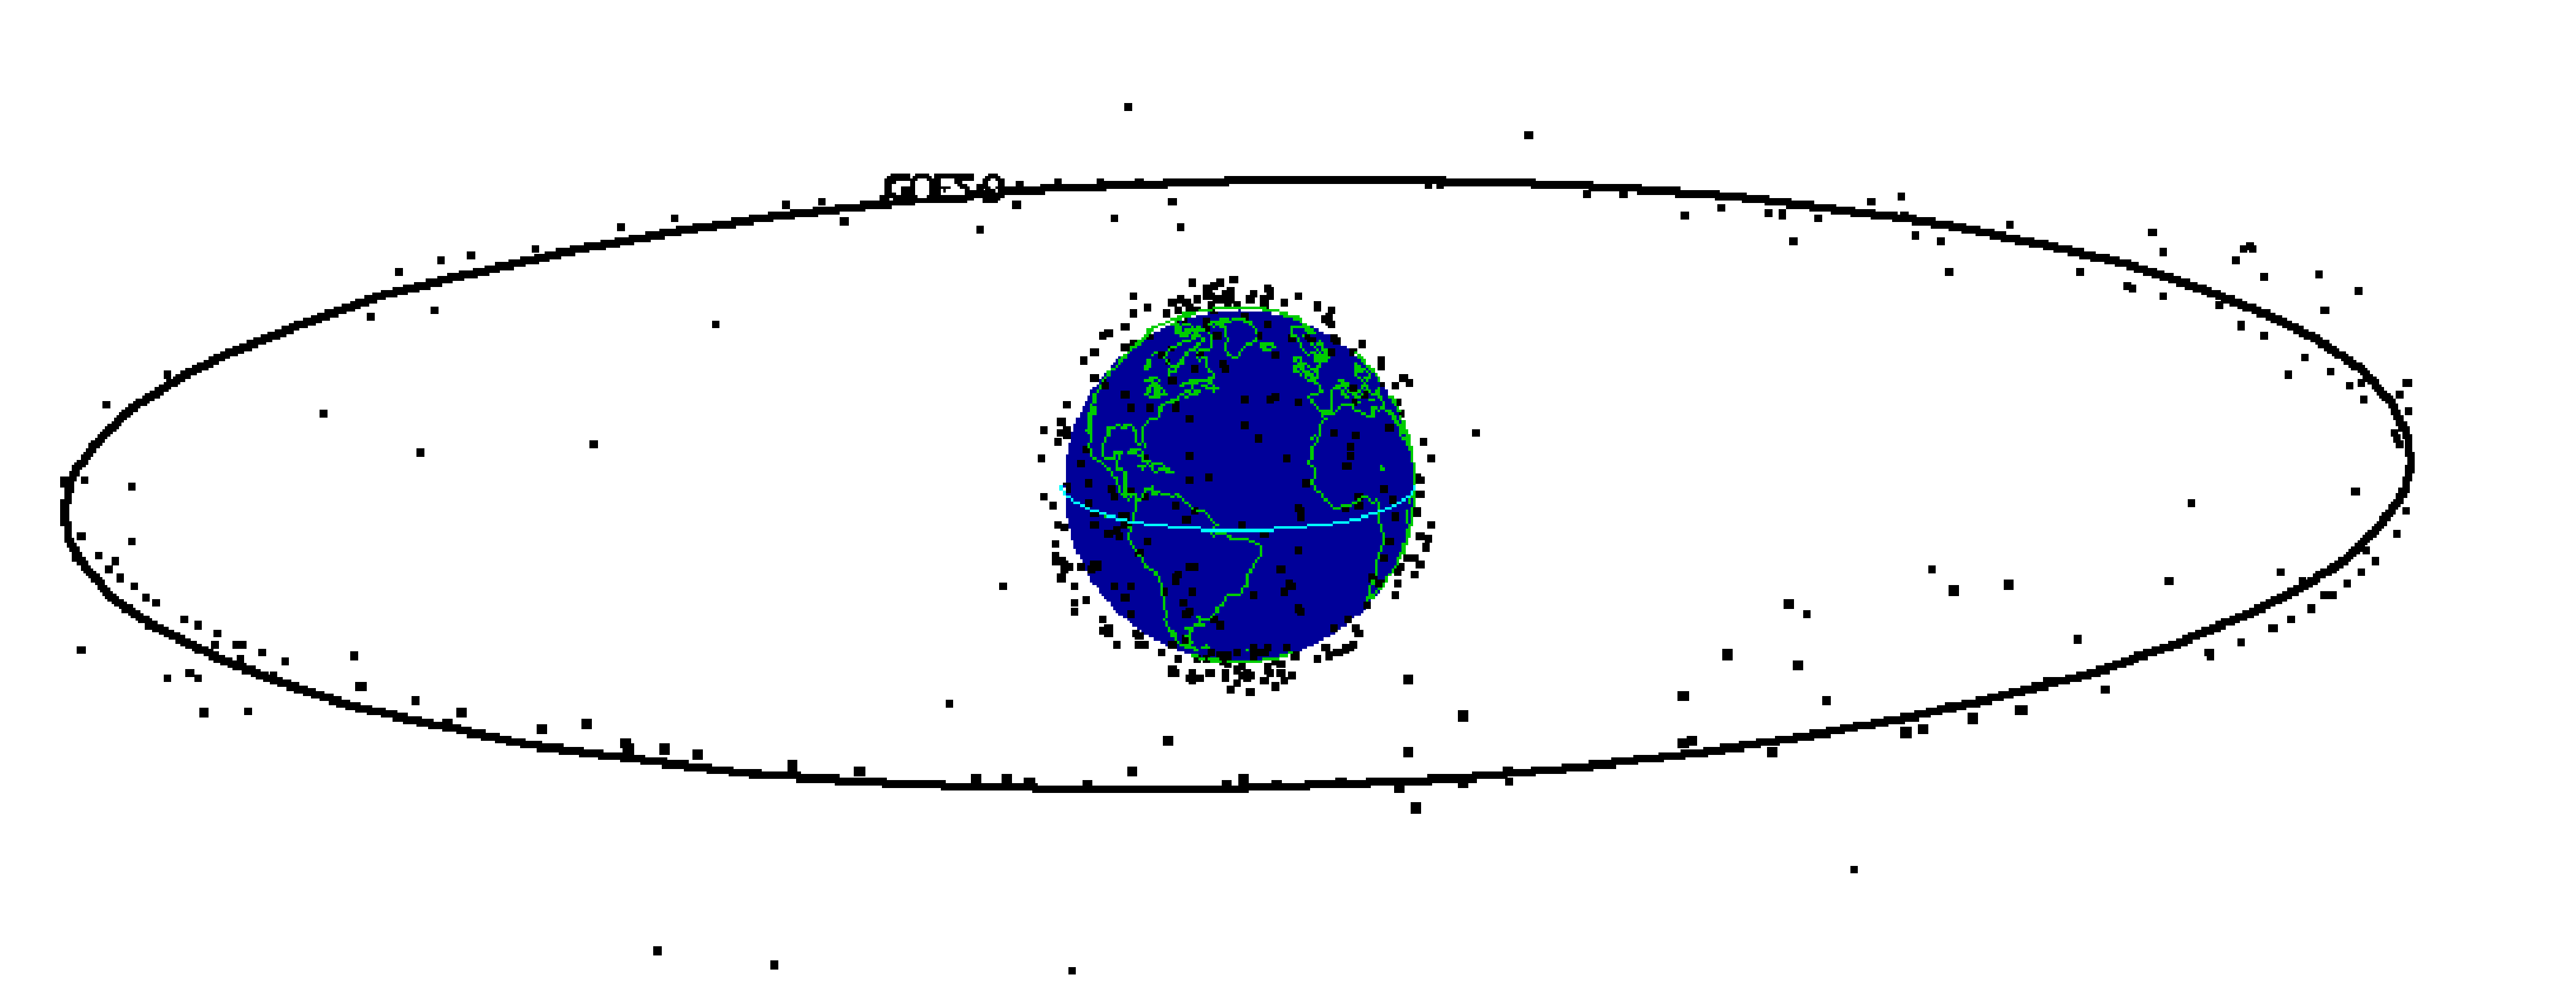
\includegraphics[width=10cm]{figs/satellites.eps}%

  \scalebox{0.8}{
  \begin{tabular}{l|c|c|c|c|c}
    Channel: & 1 & 	2 &	3 &	4 &	5 \\
    \hline \hline
    $\lambda$ [um] & 0.55-0.75 &	3.8-4.0 &	6.5-7.0 &	10.2-11.2 &11.5-12.5 \\ 
    Region & Visible & Shortwave &	Moisture &	TIR &	TIR \\
    IGFOV [km] 	&1&	4&	8 &	4 &	4 \\
    Radiometric &	5\% max  & $\le 1$ K & $\le 1$ K & $\le 1$ K & $\le 1$ K \\
  \end{tabular}
  }
\end{slide}

\begin{slide}{Row Scan Order}

  For a 3-d point lattice, \ps{X}, comprised of two spatial
  dimensions, $i$,$j$, and $t$, where $t$ corresponds to a integral
  timestamp indicator, {\bf row scan order} is the order, where for
  $\pt{x},\pt{y} \in \ps{X}$:

  \begin{gather*}
    \pt{x} \le \pt{y} \equiv
    \begin{cases}
      \pt{x}_t < \pt{y}_t & \text{ if $\pt{x}_t \ne \pt{y}_t$ }\\
      \pt{x}_i < \pt{y}_i & \text{ if $\pt{x}_t = \pt{y}_t$ }  \\
      \pt{x}_j \le \pt{y}_j & \text{ if $\pt{x}_t = \pt{y}_t$ and
        $\pt{x}_i = \pt{y}_i$ }
    \end{cases} 
  \end{gather*}
\end{slide}
\begin{slide}{Projection Definition}
  \centering
  { \fontsize{8}{8}\selectfont
\begin{verbatim}
  PROJCS["UTM 17 (WGS84) in northern hemisphere",
      GEOGCS["WGS 84",
          DATUM["WGS_1984",....
              SPHEROID["WGS 84",6378137,298.257223563,
                  AUTHORITY["EPSG",7030]],
              TOWGS84[0,0,0,0,0,0,0],
              AUTHORITY["EPSG",6326]],
          PRIMEM["Greenwich",0,AUTHORITY["EPSG",8901]],
          UNIT["DMSH",0.0174532925199433,AUTHORITY["EPSG",9108]],
          AXIS["Lat",NORTH],
          AXIS["Long",EAST],
          AUTHORITY["EPSG",4326]],
      PROJECTION["Transverse_Mercator"],
      PARAMETER["latitude_of_origin",0],
      PARAMETER["central_meridian",-81],
      PARAMETER["scale_factor",0.9996],
      PARAMETER["false_easting",500000],
      PARAMETER["false_northing",0]]
\end{verbatim}
}
\end{slide}

\begin{slide}{Reference Schema for GOES data}
  \begin{center}
    \scalebox{0.7}{\begin{picture}(0,0)%
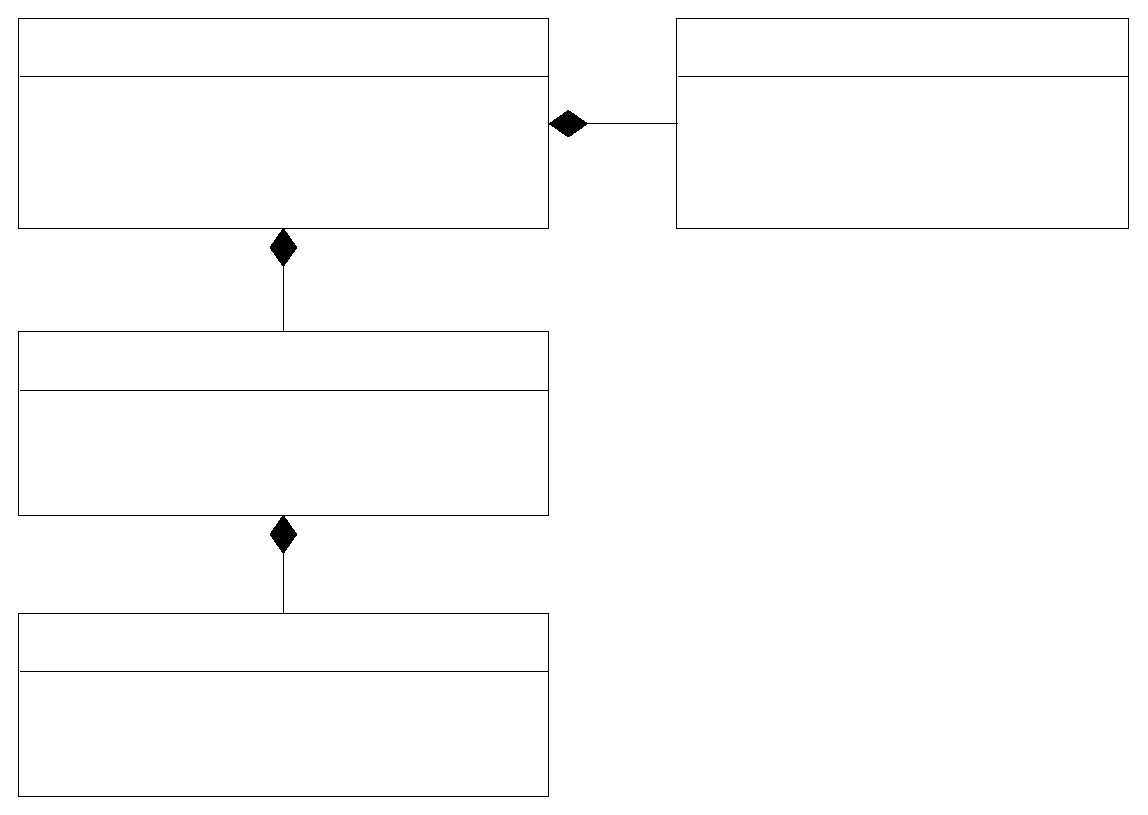
\includegraphics{figs/reference_schema.ssd.fig.eps}%
\end{picture}%
\setlength{\unitlength}{3947sp}%
%
\begingroup\makeatletter\ifx\SetFigFontNFSS\undefined%
\gdef\SetFigFontNFSS#1#2#3#4#5{%
  \reset@font\fontsize{#1}{#2pt}%
  \fontfamily{#3}\fontseries{#4}\fontshape{#5}%
  \selectfont}%
\fi\endgroup%
\begin{picture}(8904,6249)(717,-5908)
\put(7801, 37){\makebox(0,0)[b]{\smash{{\SetFigFontNFSS{10}{12.0}{\rmdefault}{\mddefault}{\updefault}Frame Info}}}}
\put(6061,-353){\makebox(0,0)[lb]{\smash{{\SetFigFontNFSS{10}{12.0}{\rmdefault}{\mddefault}{\updefault}TINFS: Frame Start Date/Time}}}}
\put(6061,-579){\makebox(0,0)[lb]{\smash{{\SetFigFontNFSS{10}{12.0}{\rmdefault}{\mddefault}{\updefault}IFRAM: Identifier}}}}
\put(6053,-803){\makebox(0,0)[lb]{\smash{{\SetFigFontNFSS{10}{12.0}{\rmdefault}{\mddefault}{\updefault}End Timestamp}}}}
\put(6061,-1029){\makebox(0,0)[lb]{\smash{{\SetFigFontNFSS{10}{12.0}{\rmdefault}{\mddefault}{\updefault}BBOX: $\ps{F} \in \Bbb{Z}^3$}}}}
\put(6061,-1253){\makebox(0,0)[lb]{\smash{{\SetFigFontNFSS{10}{12.0}{\rmdefault}{\mddefault}{\updefault}IMC-Identifier}}}}
\put(2851, 14){\makebox(0,0)[b]{\smash{{\SetFigFontNFSS{10}{12.0}{\rmdefault}{\mddefault}{\updefault}Geostream Image}}}}
\put(789,-353){\makebox(0,0)[lb]{\smash{{\SetFigFontNFSS{10}{12.0}{\rmdefault}{\mddefault}{\updefault}$\vs{C}_n$: Radiance}}}}
\put(796,-579){\makebox(0,0)[lb]{\smash{{\SetFigFontNFSS{10}{12.0}{\rmdefault}{\mddefault}{\updefault}$\ps{X}_n \in \vs{Z}^3: X(r,c,F)$}}}}
\put(789,-803){\makebox(0,0)[lb]{\smash{{\SetFigFontNFSS{10}{12.0}{\rmdefault}{\mddefault}{\updefault}$r,c,F$ = row,column,IFRAM}}}}
\put(789,-1029){\makebox(0,0)[lb]{\smash{{\SetFigFontNFSS{10}{12.0}{\rmdefault}{\mddefault}{\updefault}srs: spatial reference frame}}}}
\put(789,-1253){\makebox(0,0)[lb]{\smash{{\SetFigFontNFSS{10}{12.0}{\rmdefault}{\mddefault}{\updefault}mat: transformation matrix}}}}
\put(2851,-2469){\makebox(0,0)[b]{\smash{{\SetFigFontNFSS{10}{12.0}{\rmdefault}{\mddefault}{\updefault}Geostream Frame}}}}
\put(789,-2859){\makebox(0,0)[lb]{\smash{{\SetFigFontNFSS{10}{12.0}{\rmdefault}{\mddefault}{\updefault}$\vs{C}_n$: Radiance}}}}
\put(796,-3083){\makebox(0,0)[lb]{\smash{{\SetFigFontNFSS{10}{12.0}{\rmdefault}{\mddefault}{\updefault}$\ps{X}_n \in \vs{Z}^3: X(r,c,F)$}}}}
\put(789,-3309){\makebox(0,0)[lb]{\smash{{\SetFigFontNFSS{10}{12.0}{\rmdefault}{\mddefault}{\updefault}$F$ is constant}}}}
\put(789,-3533){\makebox(0,0)[lb]{\smash{{\SetFigFontNFSS{10}{12.0}{\rmdefault}{\mddefault}{\updefault}mat: transformation matrix}}}}
\put(3061,-1569){\makebox(0,0)[b]{\smash{{\SetFigFontNFSS{10}{12.0}{\rmdefault}{\mddefault}{\updefault}1}}}}
\put(2641,-2093){\makebox(0,0)[b]{\smash{{\SetFigFontNFSS{10}{12.0}{\rmdefault}{\mddefault}{\updefault}1..n}}}}
\put(2851,-4719){\makebox(0,0)[b]{\smash{{\SetFigFontNFSS{10}{12.0}{\rmdefault}{\mddefault}{\updefault}Geostream Row}}}}
\put(789,-5109){\makebox(0,0)[lb]{\smash{{\SetFigFontNFSS{10}{12.0}{\rmdefault}{\mddefault}{\updefault}$\vs{C}_n$: Radiance}}}}
\put(796,-5333){\makebox(0,0)[lb]{\smash{{\SetFigFontNFSS{10}{12.0}{\rmdefault}{\mddefault}{\updefault}$\ps{X}_n \in \vs{Z}^3: X(r,c,F)$}}}}
\put(789,-5559){\makebox(0,0)[lb]{\smash{{\SetFigFontNFSS{10}{12.0}{\rmdefault}{\mddefault}{\updefault}$F,r$ are constant}}}}
\put(789,-5783){\makebox(0,0)[lb]{\smash{{\SetFigFontNFSS{10}{12.0}{\rmdefault}{\mddefault}{\updefault}mat: transformation matrix}}}}
\put(3061,-3863){\makebox(0,0)[b]{\smash{{\SetFigFontNFSS{10}{12.0}{\rmdefault}{\mddefault}{\updefault}1}}}}
\put(2641,-4343){\makebox(0,0)[b]{\smash{{\SetFigFontNFSS{10}{12.0}{\rmdefault}{\mddefault}{\updefault}1..n}}}}
\put(5131,-729){\makebox(0,0)[b]{\smash{{\SetFigFontNFSS{10}{12.0}{\ttdefault}{\mddefault}{\updefault}1}}}}
\put(5701,-436){\makebox(0,0)[b]{\smash{{\SetFigFontNFSS{10}{12.0}{\ttdefault}{\mddefault}{\updefault}1..n}}}}
\end{picture}%
}
  \end{center}
\end{slide}

\begin{slide}{Reference Query trees}
  \centering
%  \newcommand{\Tb}[1]{ \Tr{\psframebox{\rule{0pt}{9pt}#1}} }
\scalebox{0.8}{
  \begin{tabular}{ccccc}
    \raisebox{\depth}{
      \pstree[nodesep=2pt,levelsep=30pt]{\TR{\im{VIS}}}{
        \pstree{\Tb{$|_{\ps{NA}}$}}{
          \TR{Q}
        }
      }} &
    \pstree[treemode=U,nodesep=2pt,levelsep=30pt]{\TR{Q}}{
      \pstree[treemode=U]{\Tb{$|_{NA}$}}{
        \pstree[treemode=U]{\Tcircle{/}}{
          \pstree[treemode=U]{\Tcircle{+}}{
            \TR[name=VIS]{\im{VIS}}
            \TR[name=IR]{\im{IR}}
          }
          \Tcircle[name=minus]{-}
          \ncline{VIS}{minus}
          \ncline{IR}{minus}
        }
      }
    } &
    \raisebox{\depth}{ \lnd{Q} \psrnd{CA} \gtnd{UTM} \ind{VIS} \tree} &
    \raisebox{\depth}{ \lnd{Q} \psrnd{< \pt{d}} \psrnd{CA} \gtnd{UTM} \ind{VIS} \tree} &
    \raisebox{\depth} { \lnd{Q} \psrnd{@t} \psrnd{NA} \ind{VIS} \tree} \\
    $\im{VIS}|_{\ps{NA}}$ &
    $\frac{\im{IR}-\im{VIS}}{\im{VIS}+\im{IR}}|_{\ps{NA}}$ &
    $\im{VIS}\circ~UTM~|_{\ps{CA}}$ &
    $\im{VIS}\circ~UTM~|_{\ps{CA}}|_{\ps{<\pt{d}}}$ &
    $\im{VIS}|_{\ps{NA}}|_{\ps{@t}}$
  \end{tabular}
}
\end{slide}

\begin{slide}{Memory Reuse}
  \centering
  \begin{tabular}{ccc}
    \scalebox{0.6}{\begin{picture}(0,0)%
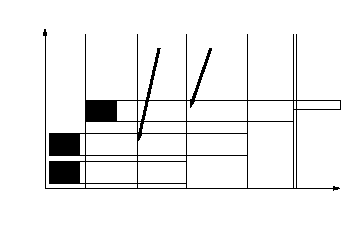
\includegraphics{figs/NDVI-r-1.fig.eps}%
\end{picture}%
\setlength{\unitlength}{4144sp}%
%
\begingroup\makeatletter\ifx\SetFigFontNFSS\undefined%
\gdef\SetFigFontNFSS#1#2#3#4#5{%
  \reset@font\fontsize{#1}{#2pt}%
  \fontfamily{#3}\fontseries{#4}\fontshape{#5}%
  \selectfont}%
\fi\endgroup%
\begin{picture}(2492,1547)(-14,-642)
\put(149,296){\rotatebox{90.0}{\makebox(0,0)[lb]{\smash{{\SetFigFontNFSS{5}{6.0}{\familydefault}{\mddefault}{\updefault}{\color[rgb]{0,0,0}Size}%
}}}}}
\put(1326,-627){\makebox(0,0)[lb]{\smash{{\SetFigFontNFSS{5}{6.0}{\familydefault}{\mddefault}{\updefault}{\color[rgb]{0,0,0}Time}%
}}}}
\put(  1,-92){\makebox(0,0)[lb]{\smash{{\SetFigFontNFSS{5}{6.0}{\familydefault}{\mddefault}{\updefault}{\color[rgb]{0,0,0}\im{VIS}}%
}}}}
\put(  1,-302){\makebox(0,0)[lb]{\smash{{\SetFigFontNFSS{5}{6.0}{\familydefault}{\mddefault}{\updefault}{\color[rgb]{0,0,0}\im{IR}}%
}}}}
\put(1444,746){\makebox(0,0)[lb]{\smash{{\SetFigFontNFSS{5}{6.0}{\familydefault}{\mddefault}{\updefault}{\color[rgb]{0,0,0}$/$}%
}}}}
\put(1049,746){\makebox(0,0)[lb]{\smash{{\SetFigFontNFSS{5}{6.0}{\familydefault}{\mddefault}{\updefault}{\color[rgb]{0,0,0}$-$}%
}}}}
\put(653,746){\makebox(0,0)[lb]{\smash{{\SetFigFontNFSS{5}{6.0}{\familydefault}{\mddefault}{\updefault}{\color[rgb]{0,0,0}$+$}%
}}}}
\put(1794,746){\makebox(0,0)[lb]{\smash{{\SetFigFontNFSS{5}{6.0}{\familydefault}{\mddefault}{\updefault}{\color[rgb]{0,0,0}$|_\ps{NA}$}%
}}}}
\put(2206,344){\makebox(0,0)[lb]{\smash{{\SetFigFontNFSS{5}{6.0}{\familydefault}{\mddefault}{\updefault}{\color[rgb]{0,0,0}\im{Q}}%
}}}}
\end{picture}%
} & 
    \scalebox{0.6}{\input{figs/NDVI-r-2.fig.tex}} & 
    \scalebox{0.6}{\begin{picture}(0,0)%
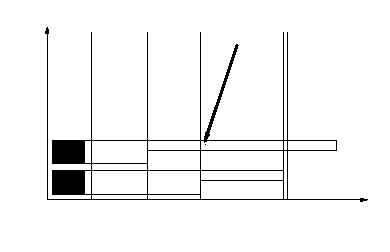
\includegraphics{figs/NDVI-r-3.fig.eps}%
\end{picture}%
\setlength{\unitlength}{4144sp}%
%
\begingroup\makeatletter\ifx\SetFigFontNFSS\undefined%
\gdef\SetFigFontNFSS#1#2#3#4#5{%
  \reset@font\fontsize{#1}{#2pt}%
  \fontfamily{#3}\fontseries{#4}\fontshape{#5}%
  \selectfont}%
\fi\endgroup%
\begin{picture}(2699,1662)(-14,-764)
\put(161,251){\rotatebox{90.0}{\makebox(0,0)[lb]{\smash{{\SetFigFontNFSS{5}{6.0}{\familydefault}{\mddefault}{\updefault}{\color[rgb]{0,0,0}Size}%
}}}}}
\put(1437,-749){\makebox(0,0)[lb]{\smash{{\SetFigFontNFSS{5}{6.0}{\familydefault}{\mddefault}{\updefault}{\color[rgb]{0,0,0}Time}%
}}}}
\put(  1,-170){\makebox(0,0)[lb]{\smash{{\SetFigFontNFSS{5}{6.0}{\familydefault}{\mddefault}{\updefault}{\color[rgb]{0,0,0}\im{VIS}}%
}}}}
\put(  1,-396){\makebox(0,0)[lb]{\smash{{\SetFigFontNFSS{5}{6.0}{\familydefault}{\mddefault}{\updefault}{\color[rgb]{0,0,0}\im{IR}}%
}}}}
\put(582,739){\makebox(0,0)[lb]{\smash{{\SetFigFontNFSS{5}{6.0}{\familydefault}{\mddefault}{\updefault}{\color[rgb]{0,0,0}$|_\ps{NA}$}%
}}}}
\put(1035,739){\makebox(0,0)[lb]{\smash{{\SetFigFontNFSS{5}{6.0}{\familydefault}{\mddefault}{\updefault}{\color[rgb]{0,0,0}$|_\ps{NA}$}%
}}}}
\put(1490,739){\makebox(0,0)[lb]{\smash{{\SetFigFontNFSS{5}{6.0}{\familydefault}{\mddefault}{\updefault}{\color[rgb]{0,0,0}$f(\im{VIS},\im{IR})$}%
}}}}
\put(2116, 29){\makebox(0,0)[lb]{\smash{{\SetFigFontNFSS{5}{6.0}{\familydefault}{\mddefault}{\updefault}{\color[rgb]{0,0,0}\im{Q}}%
}}}}
\end{picture}%
} \\
  {\tiny No optimizations} & 
  {\tiny Merge induced operations} &    
  {\tiny Distribute Selections} \\
\end{tabular}

\vspace*{0.5cm}
{\fontsize{8}{8}\selectfont
  \begin{tabular}{c|c|c|c}
    Exectuion & Creation & Max Size & Size-Time \\
    \hline \hline
    $C_{m} + 3 m C_{\gamma} + C_{|}$ & 1 & 3 & $3 C_{m} + 8 m C_{\gamma} + C_{|}$ \\
    $3 m C_{\gamma} + C_{|}$ & 0 & 2 & $6 m C_{\gamma} + C_{|}$ \\
    $3 s m C_{\gamma} + 2 C_{|}$ & 0 & 2s & $2 s m C_{\gamma} + (3+s) C_{|}$ 
  \end{tabular}
}
\end{slide}

\begin{slide}{Multi-Query Optimization}

  \vspace*{0.5cm}

  A {\blue Query Execution Graph \ac{QEG}}, is an acyclic directed
  graph $QEG = \{V,A\}$ that represents the operations to execute all
  active queries within the \ac{dsms}.  The nodes, $V$, correspond to
  individual operators within the system, and the arcs $A$, correspond
  to data paths from one operator to another.  Nodes are annotated to
  include operator costs, and arcs include the defined point sets that
  the data may include.

  \vspace*{1cm}

  A {\blue Query Execution Plan \ac{QEP}} is a combination of a
  \ac{QEG}, plus an ordering on the nodes of $V$, which satisfies the
  partial ordering imposed by a topological sort of the \ac{QEG}.
  
\end{slide}

\begin{slide}[R]{Previous Work}
  \begin{minipage}[t]{6cm}
  \begin{itemize}
  \item Multi-query optimization
    \begin{itemize}
    \item Grouped Filters
    \item Query Index
    \end{itemize}
  \item Spatial Indices
    \begin{itemize}
    \item R-tree variants
    \item Segment trees
    \item Grids
    \end{itemize}
  \item Incremental Schemes
  \item Regions of validity
  \end{itemize}
  \end{minipage}
  \begin{minipage}[t]{5cm}
    \vspace*{0pt}
    \scalebox{0.6}{\begin{picture}(0,0)%
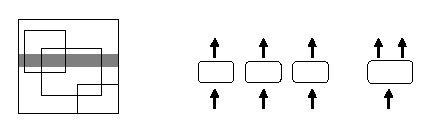
\includegraphics{figs/query-eval.fig.eps}%
\end{picture}%
\setlength{\unitlength}{4144sp}%
%
\begingroup\makeatletter\ifx\SetFigFont\undefined%
\gdef\SetFigFont#1#2#3#4#5{%
  \reset@font\fontsize{#1}{#2pt}%
  \fontfamily{#3}\fontseries{#4}\fontshape{#5}%
  \selectfont}%
\fi\endgroup%
\begin{picture}(3030,792)(-11,59)
\put(2686,419){\makebox(0,0)[lb]{\smash{{\SetFigFont{5}{6.0}{\familydefault}{\mddefault}{\updefault}{\color[rgb]{0,0,0}\dct}%
}}}}
\put( 91,659){\makebox(0,0)[lb]{\smash{{\SetFigFont{5}{6.0}{\familydefault}{\mddefault}{\updefault}{\color[rgb]{0,0,0}$R_1$}%
}}}}
\put(226,299){\makebox(0,0)[lb]{\smash{{\SetFigFont{5}{6.0}{\familydefault}{\mddefault}{\updefault}{\color[rgb]{0,0,0}$R_2$}%
}}}}
\put(496,164){\makebox(0,0)[lb]{\smash{{\SetFigFont{5}{6.0}{\familydefault}{\mddefault}{\updefault}{\color[rgb]{0,0,0}$R_3$}%
}}}}
\put(811,479){\makebox(0,0)[lb]{\smash{{\SetFigFont{5}{6.0}{\familydefault}{\mddefault}{\updefault}{\color[rgb]{0,0,0}RSI}%
}}}}
\put(1416,738){\makebox(0,0)[lb]{\smash{{\SetFigFont{5}{6.0}{\familydefault}{\mddefault}{\updefault}{\color[rgb]{0,0,0}$Q_1$}%
}}}}
\put(1787,738){\makebox(0,0)[lb]{\smash{{\SetFigFont{5}{6.0}{\familydefault}{\mddefault}{\updefault}{\color[rgb]{0,0,0}$Q_2$}%
}}}}
\put(2157,738){\makebox(0,0)[lb]{\smash{{\SetFigFont{5}{6.0}{\familydefault}{\mddefault}{\updefault}{\color[rgb]{0,0,0}$Q_3$}%
}}}}
\put(1388,404){\makebox(0,0)[lb]{\smash{{\SetFigFont{5}{6.0}{\familydefault}{\mddefault}{\updefault}{\color[rgb]{0,0,0}$R_1$}%
}}}}
\put(1748,404){\makebox(0,0)[lb]{\smash{{\SetFigFont{5}{6.0}{\familydefault}{\mddefault}{\updefault}{\color[rgb]{0,0,0}$R_2$}%
}}}}
\put(2108,404){\makebox(0,0)[lb]{\smash{{\SetFigFont{5}{6.0}{\familydefault}{\mddefault}{\updefault}{\color[rgb]{0,0,0}$R_3$}%
}}}}
\put(1441, 74){\makebox(0,0)[lb]{\smash{{\SetFigFont{5}{6.0}{\familydefault}{\mddefault}{\updefault}{\color[rgb]{0,0,0}RSI}%
}}}}
\put(1801, 74){\makebox(0,0)[lb]{\smash{{\SetFigFont{5}{6.0}{\familydefault}{\mddefault}{\updefault}{\color[rgb]{0,0,0}RSI}%
}}}}
\put(2161, 74){\makebox(0,0)[lb]{\smash{{\SetFigFont{5}{6.0}{\familydefault}{\mddefault}{\updefault}{\color[rgb]{0,0,0}RSI}%
}}}}
\put(2746, 74){\makebox(0,0)[lb]{\smash{{\SetFigFont{5}{6.0}{\familydefault}{\mddefault}{\updefault}{\color[rgb]{0,0,0}RSI}%
}}}}
\put(2656,749){\makebox(0,0)[lb]{\smash{{\SetFigFont{5}{6.0}{\familydefault}{\mddefault}{\updefault}{\color[rgb]{0,0,0}$Q_1'$}%
}}}}
\put(2836,749){\makebox(0,0)[lb]{\smash{{\SetFigFont{5}{6.0}{\familydefault}{\mddefault}{\updefault}{\color[rgb]{0,0,0}$Q_2'$}%
}}}}
\end{picture}%
}
  \end{minipage}
\end{slide}


\begin{slide}[R]{Polar Orbiting Weather Satellites }
\input{presentation/motivation-poes.fig.tex}
\end{slide}

\begin{slide}{DCT - Box Move}
  \centering
  \scalebox{0.8}{\begin{picture}(0,0)%
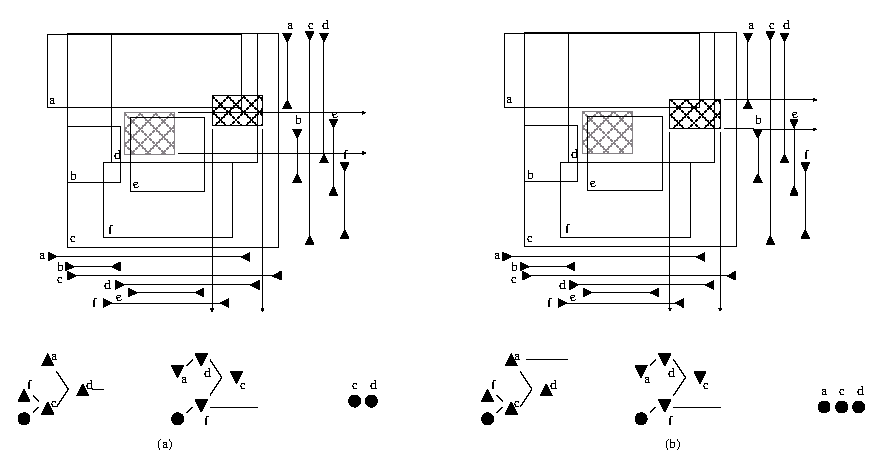
\includegraphics{figs/move.fig.eps}%
\end{picture}%
\setlength{\unitlength}{4144sp}%
%
\begingroup\makeatletter\ifx\SetFigFont\undefined%
\gdef\SetFigFont#1#2#3#4#5{%
  \reset@font\fontsize{#1}{#2pt}%
  \fontfamily{#3}\fontseries{#4}\fontshape{#5}%
  \selectfont}%
\fi\endgroup%
\begin{picture}(6478,3331)(191,-2492)
\put(5457,-1512){\makebox(0,0)[lb]{\smash{{\SetFigFont{7}{8.4}{\familydefault}{\mddefault}{\updefault}{\color[rgb]{0,0,0}\wxx}%
}}}}
\put(5074,-1512){\makebox(0,0)[lb]{\smash{{\SetFigFont{7}{8.4}{\familydefault}{\mddefault}{\updefault}{\color[rgb]{0,0,0}\wxn}%
}}}}
\put(6337,182){\makebox(0,0)[lb]{\smash{{\SetFigFont{7}{8.4}{\familydefault}{\mddefault}{\updefault}{\color[rgb]{0,0,0}\wyx}%
}}}}
\put(6337,-42){\makebox(0,0)[lb]{\smash{{\SetFigFont{7}{8.4}{\familydefault}{\mddefault}{\updefault}{\color[rgb]{0,0,0}\wyn}%
}}}}
\put(901,-1771){\makebox(0,0)[lb]{\smash{{\SetFigFont{7}{8.4}{\rmdefault}{\mddefault}{\updefault}{\color[rgb]{0,0,0}\Yn}%
}}}}
\put(2071,-2176){\makebox(0,0)[lb]{\smash{{\SetFigFont{7}{8.4}{\rmdefault}{\mddefault}{\updefault}{\color[rgb]{0,0,0}\wyn}%
}}}}
\put(2026,-1771){\makebox(0,0)[lb]{\smash{{\SetFigFont{7}{8.4}{\rmdefault}{\mddefault}{\updefault}{\color[rgb]{0,0,0}\Yx}%
}}}}
\put(901,-2041){\makebox(0,0)[lb]{\smash{{\SetFigFont{7}{8.4}{\rmdefault}{\mddefault}{\updefault}{\color[rgb]{0,0,0}\wyx}%
}}}}
\put(2746,-1771){\makebox(0,0)[lb]{\smash{{\SetFigFont{7}{8.4}{\rmdefault}{\mddefault}{\updefault}{\color[rgb]{0,0,0}\A}%
}}}}
\put(4433,-1816){\makebox(0,0)[lb]{\smash{{\SetFigFont{7}{8.4}{\rmdefault}{\mddefault}{\updefault}{\color[rgb]{0,0,0}\wyx}%
}}}}
\put(4433,-2266){\makebox(0,0)[lb]{\smash{{\SetFigFont{7}{8.4}{\rmdefault}{\mddefault}{\updefault}{\color[rgb]{0,0,0}\Yn}%
}}}}
\put(5603,-2176){\makebox(0,0)[lb]{\smash{{\SetFigFont{7}{8.4}{\rmdefault}{\mddefault}{\updefault}{\color[rgb]{0,0,0}\wyn}%
}}}}
\put(5558,-1771){\makebox(0,0)[lb]{\smash{{\SetFigFont{7}{8.4}{\rmdefault}{\mddefault}{\updefault}{\color[rgb]{0,0,0}\Yx}%
}}}}
\put(6323,-1771){\makebox(0,0)[lb]{\smash{{\SetFigFont{7}{8.4}{\rmdefault}{\mddefault}{\updefault}{\color[rgb]{0,0,0}\A}%
}}}}
\put(1618,-1514){\makebox(0,0)[lb]{\smash{{\SetFigFont{6}{7.2}{\familydefault}{\mddefault}{\updefault}{\color[rgb]{0,0,0}\wxn}%
}}}}
\put(2001,-1514){\makebox(0,0)[lb]{\smash{{\SetFigFont{6}{7.2}{\familydefault}{\mddefault}{\updefault}{\color[rgb]{0,0,0}\wxx}%
}}}}
\end{picture}%
}
\end{slide}

\end{document}

